\documentclass[10pt,journal,twoside]{IEEEtran}
% options for doc class: conference, journal, technote, peerreview, peerreviewca
% font sizes: 9pt for technote
%			 10pt for most commonly used
%			 11pt for conference
%			 12pt for computer socciety papers

% ============= math packages ===============
\usepackage[cmex10]{amsmath}

% ============= graphics and tables ====================
\usepackage{array} % improves appearance of arrays and tabular environments
\usepackage{multirow}
\usepackage{booktabs}  % Horizontal rules in tables
\renewcommand{\arraystretch}{1.3}
\usepackage[pdftex]{graphicx}
\usepackage{color}
%   declare the path(s) where your graphic files are
   \graphicspath{{PhD.Paper.Images/}}
%   and their extensions so you won't have to specify these with
%   every instance of \includegraphics
   \DeclareGraphicsExtensions{.pdf,.jpeg,.png}
%\IEEEoverridecommandlockouts % override intenationally disabled commands in coference option
\usepackage{tikz}
	\usetikzlibrary{calc,intersections}
	\usepackage{circuitikz}
	\tikzstyle{every node}=[font=\small]

%\usepackage[tight,footnotesize]{subfigure} % option 'tight' reduces white space
\usepackage[caption=false,font=footnotesize,farskip=3pt]{subfig} %
%\usepackage{fixltx2e} % helps with floats
%\usepackage{stfloats} % put floats at top and bottom of the page


% ================ other packages ====================
%\usepackage{enumitem}
%	\setlist{nolistsep}
\usepackage[detect-all]{siunitx}
\usepackage{cite}
\usepackage{url}

%\usepackage[pdftex, bookmarks, breaklinks]{hyperref}

% correct bad hyphenation here
%\hyphenation{op-tical net-works semi-conduc-tor}


\begin{document}
\bstctlcite{tj_journ_paper:BSTcontrol}
\title{MoM-based Path Loss Modelling in Rural Areas}
%\urlstyle
%%\IEEEauthorblockN{} % author name
%\IEEEauthorblockA{} % author affliation

\author{Temwani~J.~Phiri,~
        David~B.~Davidson,~\IEEEmembership{Fellow,~IEEE}
        and~P.~Gideon~Wiid,~\IEEEmembership{Member,~IEEE}%
%\thanks{T.J. Phiri is a doctoral student in the Department
%of Electrical and Electronic Engineering at Stellenbosch University, South Africa, 7602 e-mail: temwanijoshua@outlook.com.}% <-this % stops a space
%\thanks{D.B. Davidson is a distinguished professor and research chair in electromagnetics for the SKA-SA and is based at Stellenbosch University}
%\thanks{P.G. Wiid is a lecturer at Stellenbosch University and leads a group specialized in EMC research and innovation}}% <-this % stops a space
%\thanks{Manuscript received April 19, 2005; revised January 11, 2007.}}
%
\thanks{The authors are with the Department of Electrical
and Electronic Engineering, Stellenbosch University, Stellenbosch 7600, South
Africa (email: temwanijoshua@outlook.com; davidson@sun.ac.za; wiidg@sun.ac.za)}}%
%
\markboth{IEEE Transactions on Antennas and Propagation}{Phiri \MakeLowercase{\textit{et al.}}: MoM-based Path Loss Modelling in Rural Areas}  %, ~Vol.~6, No.~1, March~2016}
%
\maketitle
%
\begin{abstract}
% As a general rule, do not put math, special symbols or citations in the abstract
Path loss is an important parameter for coverage mapping and spectrum management. Of special interest in this study is the modelling of path loss at low antenna heights (under \SI{10}{m}) and short ranges (less than \SI{1}{km}). This is of relevance to site evaluation of advanced radio telescopes such as MeerKAT in respect of computing RFI threshold levels and investigating coupling mechanisms. Previously, RFI thresholds have been based on free space loss predictions and are therefore inaccurate. We present a full-wave propagation model (FWPM) for path loss modelling in rural areas. Electrical characteristics of the earth are included and full antennas are modelled in order to reproduce a real world scenario. Statistical error analysis of the predictions yields an unprecedented RMSE of less than \SI{4}{dB} when compared to measurements obtained at the MeerKAT facility.
\end{abstract}
%
%\IEEEpeerreviewmaketitle % needed for peer review papers
%
\section{Introduction}
\IEEEPARstart{P}{ropagation} modelling is an important tool in the roll-out of a radio link with respect to assessing interference effects in the intervening path. The goal is to quantify the degree of signal degradation between wireless transceivers due to reflection, diffraction, scattering and other propagation phenomena besides spreading (free space) loss. Expressed as the ratio of transmitted to received power, the extent of signal attenuation is called \emph{path loss}. It is a vital parameter for coverage mapping and spectrum management \cite{Rappaport,Seybold}. Numerous path loss prediction tools utilizing theoretical, statistical, empirical and deterministic schemes have been developed over the last seven decades \cite{Phillips:Survey,Sarkar:Survey}. This highlights the significance of propagation modelling in planning various types of wireless networks. %Two broad categories exist: large-scale models where transmitter-receiver (T-R) separation distances are generally on the order of tens and hundreds of kilometres such as in broadcast services; fading or small-scale models that are concerned with fluctuations in received power over short T-R lengths such as in mobile communications and wireless local area networks (WLAN).\\ %Models involving shorter T-R distances ($<\SI{1}{km}$) are typically employed when assessing indoor propagation channels as well as outdoor propagation in urban areas.\\%
Empirical models (synthesized based on multiple measurements) tend to be most common due to their ease of implementation. However, the predictions quickly become inaccurate when they are employed in an environment other than the one on which the data is based. On the other end of the spectrum, deterministic models (derived from Maxwell's equations) offer high accuracy but require detailed information of the environment (site-specific) and are computationally expensive \cite{Sarkar:Survey,Abhayawardhana}.\\
Unsurprisingly, the vast majority of models focus on mobile radio services in urban areas as well as FM radio and television broadcast services. In the former case, propagation is typically by diffraction and scattering since there are seldom line of sight (LoS) paths. Consequently, a multipath environment exists since the received signal is a superposition of several delayed waves \cite{Harada:2002}. In this regime, multipath fading -- the variability of the wave due to constructive and destructive interference -- becomes particularly important and is accounted for using a Rayleigh probability distribution \cite{Raisanen:2003}. %a Rician probability distribution if a LoS path exists 
In the latter scenario, atmospheric scattering and refraction are the characteristic propagation effects. The physical configuration involves transmitting (base) stations that are hundreds of metres high with a coverage radius extending a few tens of kilometres. %wherefore radio waves travel a longer distance than the LoS path. Time variability must be considered due to atmospheric variations (changes in the refractive index)
One thus finds that models addressing propagation in open areas are few and far between and do not typically consider short transmitter-receiver (T-R) separation distances. With the outset of advanced and highly sensitive radio telescopes such as the Square Kilometre Array (SKA), probing signal propagation at path lengths and heights that differ from conventional telecommunication standards becomes important. Moreover, literature is thin on propagation modelling to aid electromagnetic characterization of radio astronomy facilities. %It is often supposed that under a kilometre path loss can be taken as equal to free space loss. However, this is only true when there are no obstructions in the first Fresnel zone between two transceivers.
%At path lengths less than \SI{100}{km}, losses in received signal strength are dominated by reflection and diffraction, in addition to free space loss \cite{SKAEMI}.
We thus present a novel full-wave propagation model (FWPM) based on the method of moments (MoM) for path loss predictions at T-R lengths less than \SI{1}{km}. Electrical properties of the earth are taken into account and simulated as a dielectric ground plane. Combined with the full-wave nature of the model, the ground-reflected wave is thus approximated very well. In its present form, the FWPM has no restriction on frequency but is presently limited to the range \SI{100}{} -- \SI{2700}{MHz} which falls within the mid-frequency band of the SKA. As a case study, comparisons of the FWPM predictions are made to measured data obtained at the  MeerKAT facility in South Africa's semi-desert Karoo region. Statistical error analysis yields an unprecedented \SI{3.08}{} and \SI{3.57}{dB} root mean square error for the two configurations considered.

The paper is fashioned with an overview on propagation modelling in Section \ref{Overview of Propagation Modelling} which introduces the statistical metrics used in the study. In Section \ref{The Full-Wave Propagation Model} a description of the FWPM is provided and validated by a comparison to the Friis transmission equation. The main contributions are highlighted in Section \ref{Comparison of FWPM Predictions to Measured Data} where statistical analysis is made against measured data. Concluding remarks are presented in Section \ref{Conclusion}.  

\section{Overview of Propagation Modelling}\label{Overview of Propagation Modelling}
\subsection{Basic Modelling}
In the log domain, a radio link is modelled as
\begin{equation}
\label{eqn:Pr}
P_r = \text{EIRP} + G_r - PL,
\end{equation}
% $\text{link loss} = FSL - G_t - G_r + M$, where $M$ acconts for miscellaneous losses (connector, feeder) . In free space, $P_r = P_t - \text{link loss} = P_t + G_t + G_r - FSL$
where $P_r$ is the received power in \SI{}{dBm}, $\text{EIRP} = P_t + G_t$ is the effective isotropic radiated power (\SI{}{dBm}), $G_t$ and $G_r$ are the respective transmitter and receiver gains in \SI{}{dBi}. The term $PL$ (\SI{}{dB}) is the attenuation (path loss) due to environmental and propagation effects given as
\begin{equation}
\label{eqn:PL}
PL = L_{\text{fsl}} + L_{\text{env}},
\end{equation}
where $L_{\text{fsl}}$ is the free space loss derived from the Friis transmission formula   %\footnote{The more accurate term for free space loss is \emph{spreading loss} since it is the result of the inverse square law \cite{Haslett}} %
with isotropic transceivers as the reference. The term $L_{\text{env}}$ is the loss due to reflection, diffraction or scattering depending on the propagation mode and surrounding medium\footnote{Small-scale fading effects are neglected here}. In cases where a LoS path exists and the antennas are several wavelengths above the ground, equation (\ref{eqn:PL}) can be approximated as 
\begin{equation}
\label{eqn:FSL}
PL = L_{\text{fsl}} = 10\log\left[ \left(\dfrac{4\pi d_mf}{c}\right)^2 \right],
% = 10\log\left[ \dfrac{p_t}{p_r} \right]
\end{equation}
%where the term in parenthesis is the free space loss factor with %
where f (\SI{}{Hz}) is the carrier frequency, $d_m$ (\SI{}{m}) is the T-R length and $c$ (\SI{}{m/s}) the speed of light in a vacuum.
%Free space loss is trivial to compute so that the goal of a model is to predict as accurately as possible the term $L_{rds}$
%In free space, the power at a receiver in the case of matched antennas is theoretically given by the Friis transmission formula
%\begin{equation}
%\label{eqn:Pr2}
%p_r = p_t\left(\dfrac{\lambda}{4\pi d_m}\right)^2g_tg_r = p_t\left(\dfrac{c}{4\pi d_mf}\right)^2g_tg_r,
%\end{equation}
%where $p_t$ and $p_r$ is the transmitted and received power in $W$, $\lambda$ is the wavelength ($m$) of the carrier frequency, f (\SI{}{Hz}), $d_m$ is the path length ($m$), $g_t$ and $g_r$ are the (numeric) transmitter and receiver gains, respectively. Assuming isotropic radiators, free space loss is then simply
%\begin{equation}
%\label{eqn:fsl}
%L_{fsl} = \dfrac{p_t}{p_r} = \left(\dfrac{4\pi d_mf}{c}\right)^2.
%\end{equation}
In practical units, equation (\ref{eqn:FSL}) is given as
\begin{equation}
\label{eqn:FSL2}
L_{\text{fsl}} = 20\log\left( f \right) + 20\log\left( d \right) + 32.45,
\end{equation}
with $f$ in \SI{}{MHz} and $d = 10^{-3}d_m$ in \SI{}{km}.\\
Propagation models strive to predict as accurately as possible the loss $L_{\text{env}}$. The general input parameters include frequency, antenna heights and T-R separation. More complex models such as the Longley-Rice Irregular Terrain Model (ITM) and the ITU-R P.\num{452} model can incorporate terrain data in order to account for diffraction loss due to obstructions. Effectiveness of a model in predicting path attenuation depends on its input parameters as well as whether the model is applied within its coverage range. A wide survey of various models and how they predict $PL$ is presented in \cite{Phillips:Survey}.  %Here, only two are briefly described.%
%
%Recently, a comparative study examined the efficacy of using ITU-R P.\num{1546} and ITM models at shorter path lengths and lower transceiver heights than intended \cite{Phiri}. , a comparative study was undertaken to determine the efficacy of using ITU-R P.\num{1546} and ITM models at path lengths and transceiver heights that differed from the telecommunication and broadcast standards
%\section{Standard Path Loss Models} %
%
%\subsection{The ITU-R P.\num{1546} Model\cite{P1546}}
%Recommendation P.\num{1546} of the International Telecommunication Union Radiocommunication Bureau (ITU-R) was derived empirically from measurements in a variety of climates and paths types. It is intended as an irregular terrain model for predictions spanning T-R distances of \SI{1}{} to \SI{1000}{km} and frequencies ranging from \SI{30}{} to \SI{3000}{MHz}. Implementation is via curves and tables of received E-field strength as functions of frequency, antenna heights, T-R~distances and path type (land or sea). %nominal frequencies of \SI{100}{}, \SI{600}{} and \SI{2000}{MHz} for land and sea paths and time variabilities of 1\%, 10\% and 50\%.
%If available, P.\num{1546} can be implemented with terrain data.
%%
%\subsection{The Longley-Rice Irregular Terrain Model\cite{LongleyRice}}
%The Longley-Rice Irregular Terrain Model (ITM) is a fairly detailed general purpose model for predictions in the range \SI{20}{MHz} to \SI{20}{GHz} and path lengths of \SI{1}{} to \SI{2000}{km} \cite{Hufford}. It can be used with and without terrain data. The ITM relies heavily on numerical approximations to theory in order to account for refraction losses, soil properties and climatic conditions \cite{Phillips:Stability}. The term $L_{\text{env}}$ thus takes a complicated form with respect to the number of equations that must be used. %To be precise, the ITM is an implementation of the Longley-Rice model by the National Telecommunications and Information Administration (NTIA). This package is used to generate the Longley-Rice results presented here.\\
%The ITM is available as a tool by the same name from the Institute for Telecommunication Sciences (ITS) and is also implemented in the Signal Propagation, Loss, And Terrain (\emph{SPLAT!}) analysis package.
%
\subsection{Statistical Analysis Metrics}
%First order statistics were used to evaluate the performance of the models implemented in this study.
\subsubsection{Prediction Error and Root Mean Square Error}
The prediction error, $\varepsilon$, is the most basic of metrics in evaluating a propagation  model. It is the difference between the measured %\footnote{typically the median value across multiple measurements/predictions}
and predicted value of path loss, given for a specific path as
\begin{equation}
	\label{eq:pred_error1}
	\varepsilon_{m,i}  = PL_{\text{meas}} - PL_{m,i}, \qquad i = 1,2,...,N
\end{equation}
where subscript $m$ denotes a model and and $N$ is the number of sample (frequency) points. %In describing the performance of a model it is more to quote 
The mean prediction error is simply
\begin{equation}
\bar\varepsilon_m  = \dfrac{1}{N}\sum_{i=1}^{N}\varepsilon_{m,i},
\end{equation}
and its associated standard deviation is 
\begin{equation}
\sigma_{\bar\varepsilon_m} = \sqrt{ \dfrac{\sum_{i=1}^{N} \left( \varepsilon_{m,i} - \bar\varepsilon_m \right)^2}{N-1} }.
\end{equation}
A more qualitative description of a models performance is the root mean square error (RMSE)
\begin{equation}
	\label{eq:rmse}
	\text{RMSE} = \sqrt{\dfrac{1}{N}\sum\limits_{i=1}^n \varepsilon_{m,i}^2}, \qquad (\SI{}{dB})
\end{equation}
which is a measure of deviation from the measured value. Hence the RMSE serves as the standard error of the predictions. 
%
\subsubsection{Relative Error and Accuracy}
Relative Error (RE) is the magnitude of the prediction error weighted by the measured (true) value of path loss. It is the fractional error
\begin{equation}
	\text{RE}_m = \dfrac{1}{N}\sum_{i=1}^{N}\dfrac{\left|\varepsilon_{m,i}\right|} {PL_{\text{meas}}},
\end{equation}
from which the accuracy $A_m = (1 - \text{RE}_m)\times 100$, can be calculated. The accuracy provides a confidence level for a models prediction.
%
\subsubsection{Correlation Coefficient}
Linear closeness between measurement and predictions is determined by the correlation coefficient
%The computation here is based on Pearson's product moment formulation,
\begin{equation}
	\rho = \dfrac{ \displaystyle N\sum_{i=1}^{N} PL_{\text{meas}} PL_{m,i} - \sum_{i=1}^{N} PL_{\text{meas}} \sum_{i=1}^{N} PL_{m,i} } { \displaystyle \left( N-1 \right) \sum_{i=1}^{N} PL_{\text{meas}} \sum_{i=1}^{N} PL_{m,i} }.
\end{equation}
It must be noted here that strong correlation will not necessarily mean that a model performs well but rather indicates that the model exhibits similar trends as the measured data.
%
\section{The Full-Wave Propagation Model}\label{The Full-Wave Propagation Model}
Numerical solutions to Maxwell's equations that make no \emph{a priori} physical approximations are called full-wave techniques \cite{Davidson2011}. Computational electromagnetics (CEM) offers a number of such methods which are described in several texts (see \cite{Davidson2011,Jin,Gibson}). The full-wave propagation model (FWPM) described here is based on the method of moments (MoM) implemented via the FEKO software suite. Other full-wave implementations are described in \cite{Hviid95,Yagbasan2010,Brennan2014}. % It incorporates a dielectric ground plane to simulate the influence of the earth.%
%
\subsection{The Method of Moments}
The MoM is a frequency domain full-wave technique widely used in antenna engineering as it is well suited to problems involving radiation and scattering. The method utilizes an appropriate Green function to derive an integro-differential form of Maxwell's equations. To reduce the number of unknowns and make the problem tractable computationally, a suitable boundary condition and \emph{basis functions} must be selected. This results in a system of linear equations of the form \cite{Jin},
\begin{equation}
 V_m  = \sum\limits_{n=1}^{N-1} Z_{mn} I_n, \qquad m = 1,2,...,N-1
\end{equation}
where $Z_{mn}$ is called the system matrix, $V_m$ is the source vector and $I_n$ is the unknown vector that is solved for using LU-factorization. Subscript $m$ represents sampling points while $n$ refers to source points. %A key advantage in using the MoM formulation is that discretisation is limited to the radiating or scattering structure only, since it is a \emph{source} method. In contrast, field methods require that free space be discretised as well.
The MoM implementation in the FEKO software suite includes extensions that enable the modelling of dielectrics. Of special interest here is the Sommerfeld formulation and reflection coefficient approximation that are used to simulate `real ground'.
%
\subsection{Antenna Characteristics}
The quality of radiation source data is a vital part of the FWPM. The initial intention had been to generate the data using half-wave dipoles but mismatch effects were too significant over the desired frequency range. In keeping with a relatively simple design, log-periodic dipole array (LPDA) antennas were realized in Antenna Magus and subsequently exported to FEKO. A bandwidth of \SI{160}{\%} was achieved with centre frequencies of \SI{500}{MHz} for band 1 (\SI{100}{} - \SI{900}{MHz}) and \SI{1500}{MHz} for band 2 (\SI{900}{} - \SI{2700}{MHz}). Parametrized by a spacing factor of \num{0.131}, \num{27} elements were used for each antenna. Load and input impedances were $\SI{292.19}{\Omega}$ and $\SI{200}{\Omega}$, respectively. %Simulations were ran in two bands: band \num{1} was defined as \SI{100}{} - \SI{900}{MHz} while band \num{2} covered \SI{900}{} - \SI{2700}{MHz}. The corresponding centre frequencies for the LPDA's operating in the two bands were \SI{500}{MHz} and \SI{1500}{MHz}.
Fig \ref{fig:gain_s11} shows the gain and reflection coefficient of the antennas.
\begin{figure}%
	\centering
	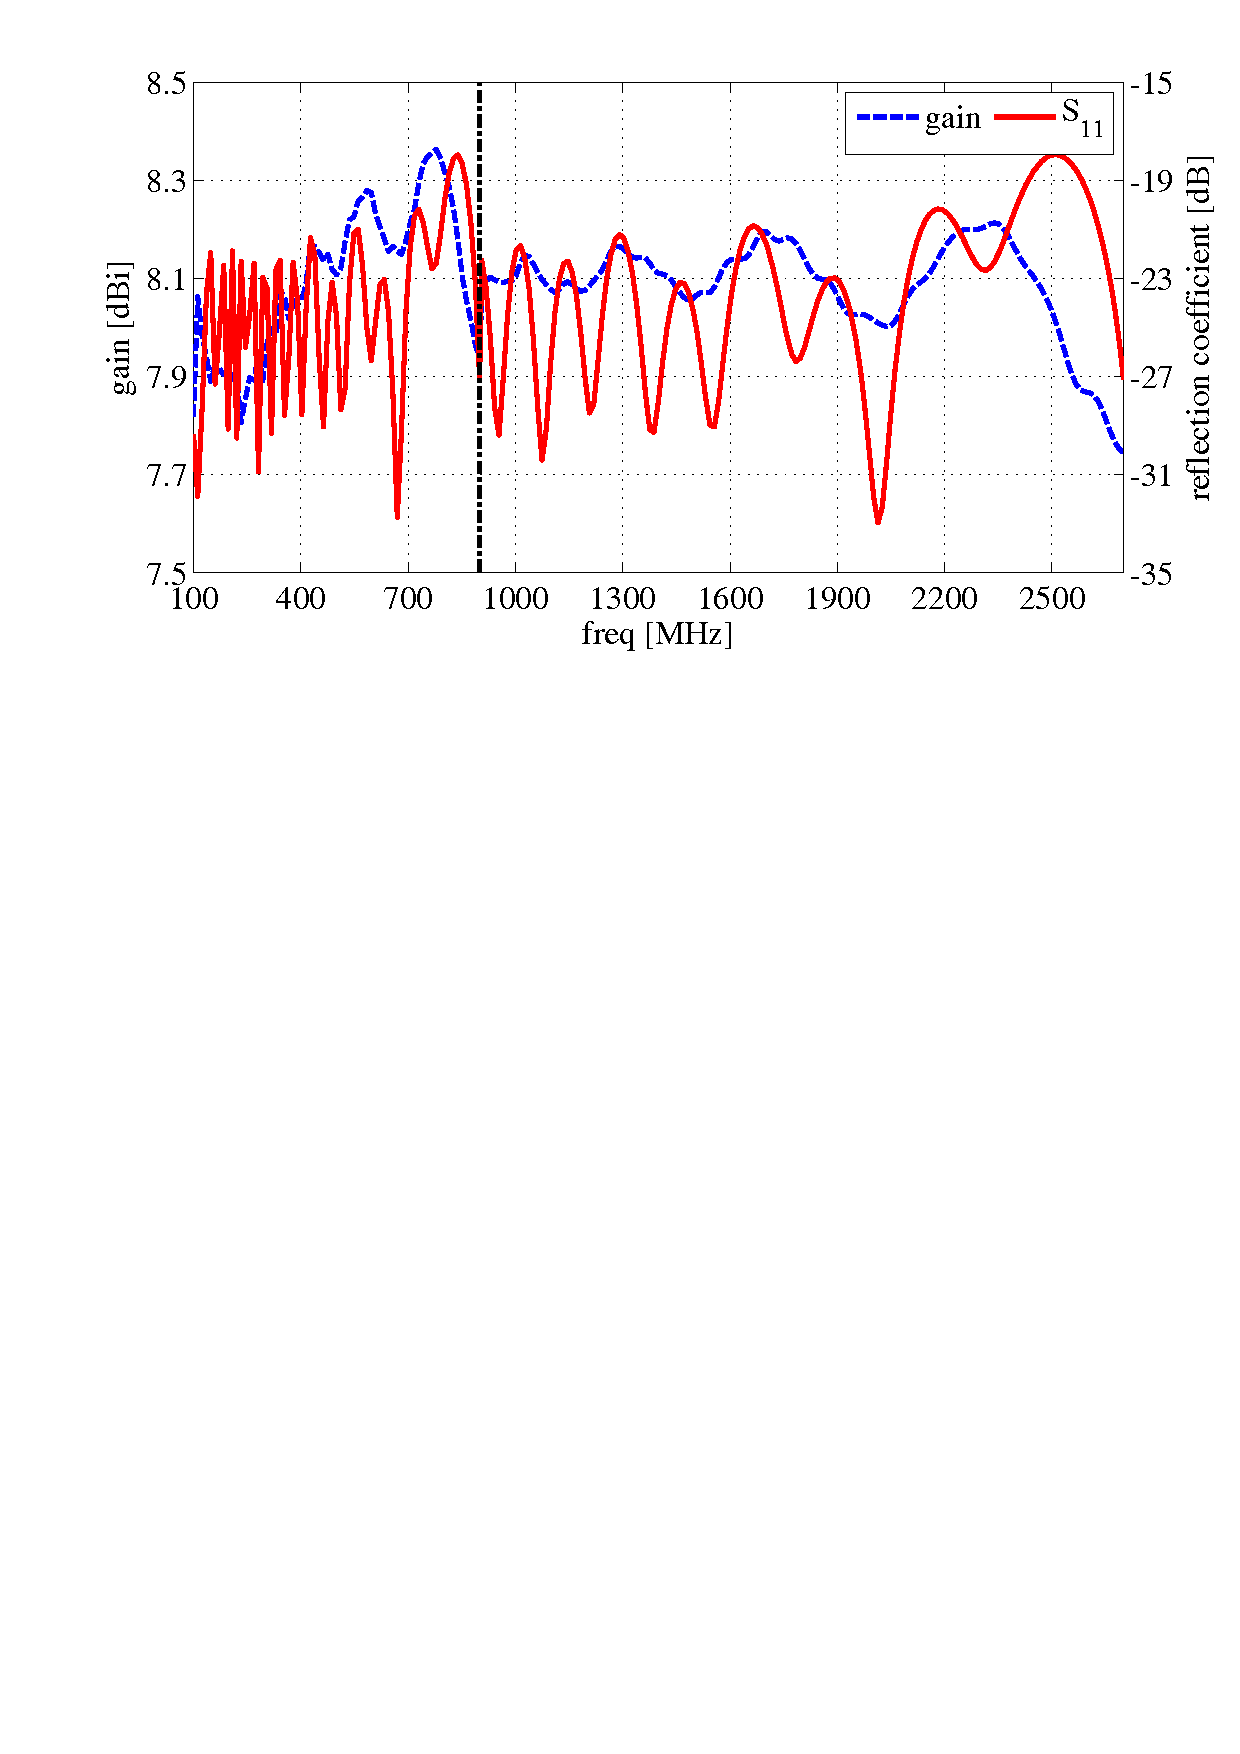
\includegraphics[width=\linewidth]{antenna_gain_s11_full}%
	\caption{Gain (\SI{}{dBi}) and reflection coefficient ($S_{11}$, \SI{}{dB}) of the LPDA's used for the FWPM simulations. The vertical dash-dot line corresponds to \SI{900}{MHz} and demarcates the transition from band \num{1} to band \num{2}.}%
	\label{fig:gain_s11}%
\end{figure}%
%
\subsection{Influence of the Ground}
%\section{Ground Wave Propagation}
Radio wave transmission that takes place in the vicinity of the earth is called ground wave propagation. Three waves are to be considered in general: surface, direct and ground-reflected waves. In many scenarios the contribution of the surface wave is negligible so that the received wave is predominantly the sum of the direct and ground-reflected waves, collectively called the space wave. In view of reflections, the electrical characteristics of the ground must be taken into account.%
%
\subsubsection{Complex Permittivity}
Given a dielectric medium of permittivity $\epsilon$\footnote{Not to be confused with prediction error, $\varepsilon$} and effective conductivity $\sigma$, the Maxwell-Ampere equation can be written as \cite{Jordan}
\begin{equation}
\nabla \times \mathbf{H} = j\omega\epsilon\mathbf{E} + \sigma \mathbf{E} = j\omega\left[ \epsilon - j\dfrac{\sigma}{\omega} \right]\mathbf{E} = j\omega\dot{\epsilon}\mathbf{E},
\end{equation}
where $\dot\epsilon$ is the complex permittivity\footnote{Strictly speaking complex permittivity is presented as $\dot{\epsilon} = \epsilon{'} - j\epsilon{''}$ \cite{Balanis:Electro}. However, in practice the macroscopic effect of the alternating field conductivity, $\omega\epsilon{''}$, is indistinguishable from the effect of $\sigma$.} that typifies the behaviour of a partially conducting dielectric. The relative complex permittivity can then be defined as
\begin{equation}
\dot\epsilon_{r} = \dfrac{\dot\epsilon}{\epsilon_0} = \epsilon_{r} - j\dfrac{\sigma}{\omega\epsilon_0} = \epsilon_{r} - jx. 
\end{equation}
Electrical characteristics of a given ground are summarized by $\dot\epsilon_{r}$. Relative permittivity and the loss term $x$ are shown in Fig \ref{fig:complex_perm} for three types of ground as provided in \cite{P527}.   
%In this work, $\dot\epsilon_{r}$ was modelled using the values recommended in \cite{P527}.
\begin{figure}
	\centering
	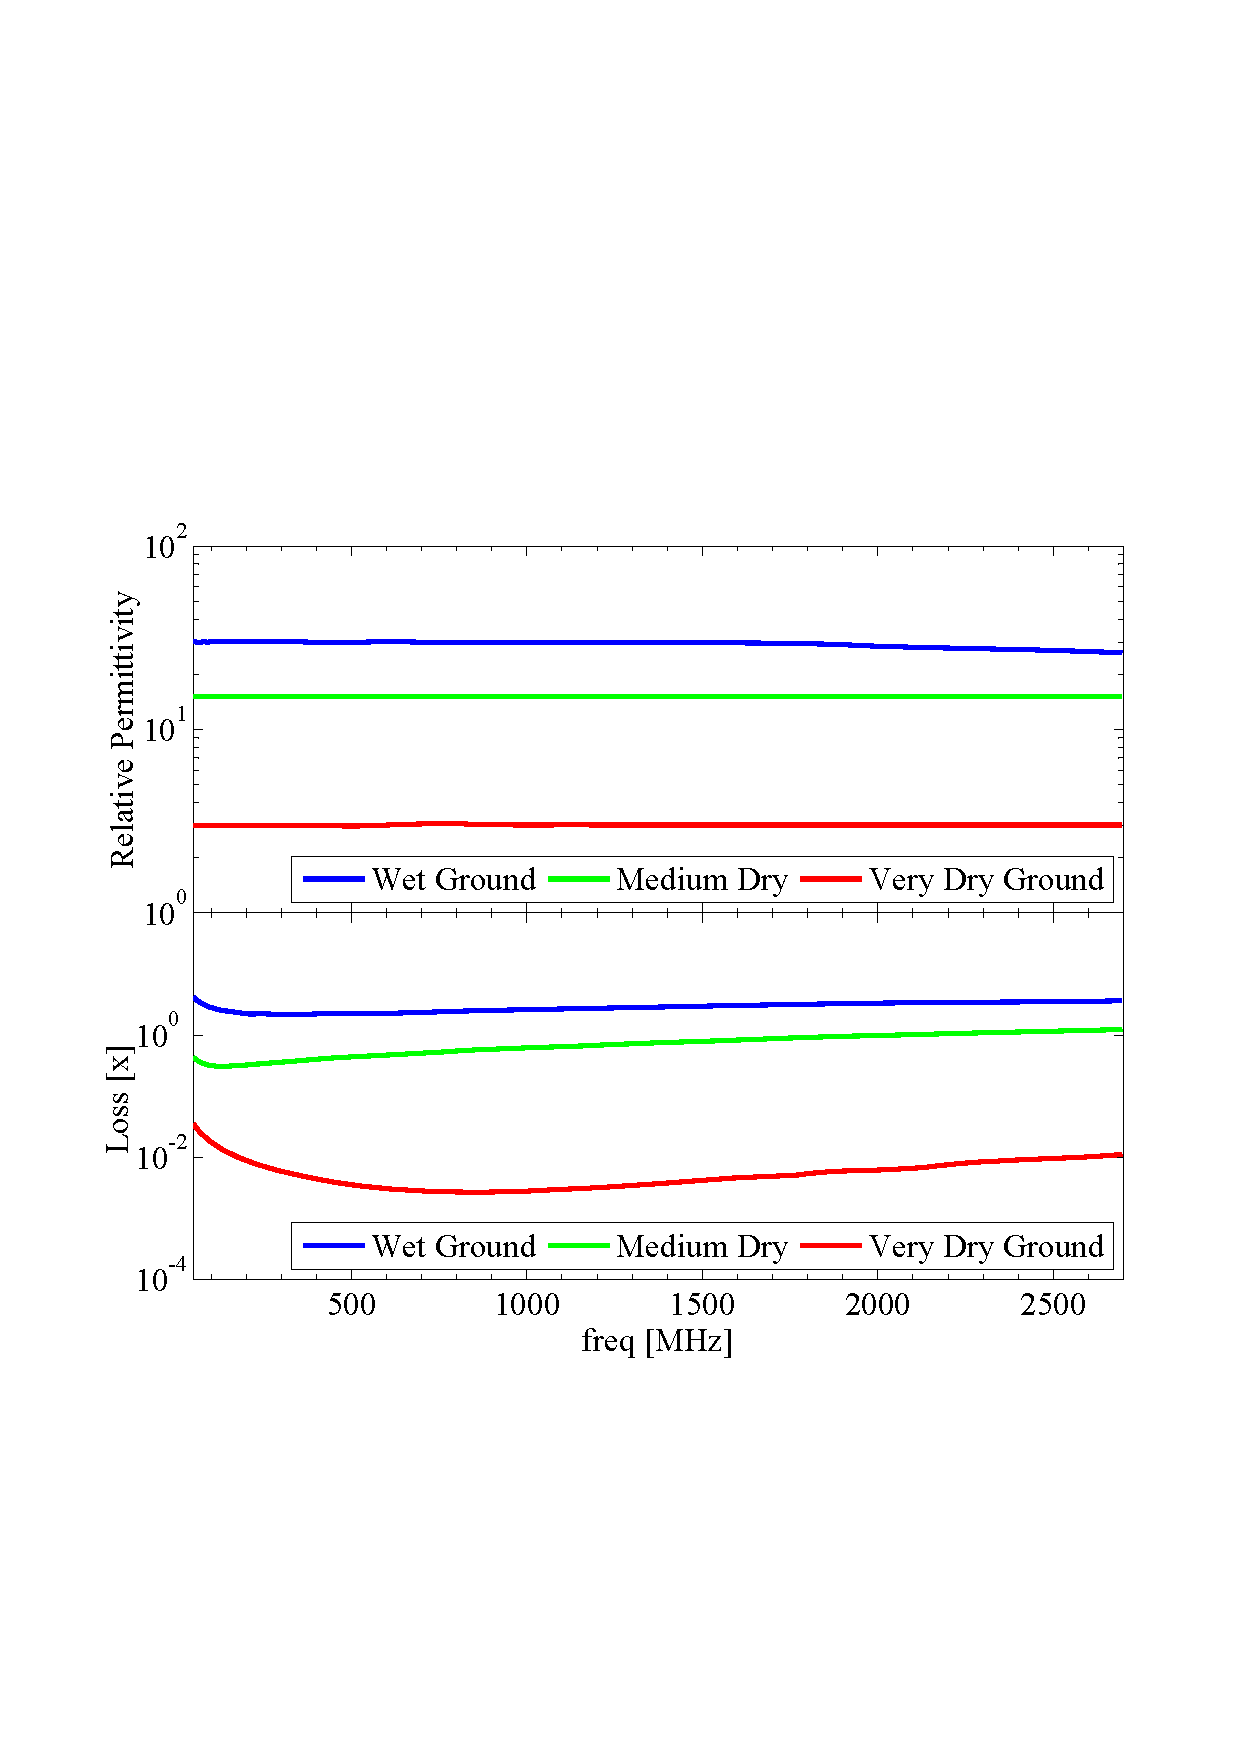
\includegraphics[width=\linewidth]{relative_permittivity_loss}%
	\caption{Relative permittivity and the loss term $x$}%
	\label{fig:complex_perm}
\end{figure}%
% affects the phase and amplitude of the received signal through the reflection coefficient.
% 
\subsubsection{Plane Earth Reflection}
% measure of roughness is given by the Rayleigh criterion \cite{Jordan}
%\begin{equation}
%R = \dfrac{4\pi\sigma\sin \phi}{\lambda}	
%\end{equation}
%where $\sigma$ is the standard deviation of the surface irregularities relative to the mean surface height, $\phi$ is the angle of incidence measured from grazing angle, $lambda$ is the wavelength.
% $R<0.1$ is considered smooth; $R>10$ is rough and the reflected wave has small magnitude
A simplified but practical approach to model ground wave propagation is  \cite{Norton37,Angelakos} %shown in equation (\ref{eq:ground_wave_set}). 
\begin{equation}
\label{eq:ground_wave_set}
\dfrac{E}{E_0} = 1 + Re^{-j\Delta\phi} + \left( 1 - R \right)Fe^{-\Delta\phi},
\end{equation}
where $E$ and $E_0$ represent the received and free space electric fields, respectively. The term $R$ represents the Fresnel reflection coefficients for vertical or horizontal polarization as shown in equations (\ref{eq:Rv}) and (\ref{eq:Rh}); $F$ is the attenuation factor (equation (\ref{eq:F})) that heavily influences the surface wave; the angle
\begin{equation}
\Delta\phi = \dfrac{\omega}{c} \left(R_2 - R_1\right)
\end{equation}
accounts for the phase difference between the direct and reflected waves where
\[ R_1 = d_m \sqrt{\left(\dfrac{h_t - h_r}{d_m} \right)^2 + 1} \]
and 
\[ R_2 = d_m \sqrt{\left(\dfrac{h_t + h_r}{d_m} \right)^2 + 1}, \]
with $d_m$ as the T-R length in metres as before. A schematic of the configuration is shown in Fig \ref{fig:reflection}.

Reflection at the interface of two media is a well known and widely discussed phenomenon. For dielectrics, the reflection coefficient will be a function of the ratio of the permittivity of the two media, polarization and angle of incidence. It can be shown that setting the relative complex permittivity of the earth to $\dot\epsilon_r$ yields \cite{Balanis:Electro,Jordan}
\begin{equation}
\label{eq:Rv}
R_v = \dfrac{ \dot\epsilon_r\sin\psi - \sqrt{\dot\epsilon_r - \cos^2\psi} }
{ \dot\epsilon_r\sin\psi + \sqrt{\dot\epsilon_r - \cos^2\psi} },
\end{equation}
%
\begin{equation}
\label{eq:Rh}
R_h = \dfrac{ \sin\psi - \sqrt{\dot\epsilon_r - \cos^2\psi} }{ \sin\psi + \sqrt{\dot\epsilon_r - \cos^2\psi} },
\end{equation}
as the %where $R_v$ and $R_h$ are
the reflection coefficients for vertical (parallel) and horizontal (perpendicular) polarizations with
\begin{equation}
\psi = 90^\circ - \theta = \arctan\left(\dfrac{h_t + h_r}{d_m} \right)
\end{equation}
as the angle of incidence (Fig~\ref{fig:reflection}). 
\begin{figure}
	\centering
	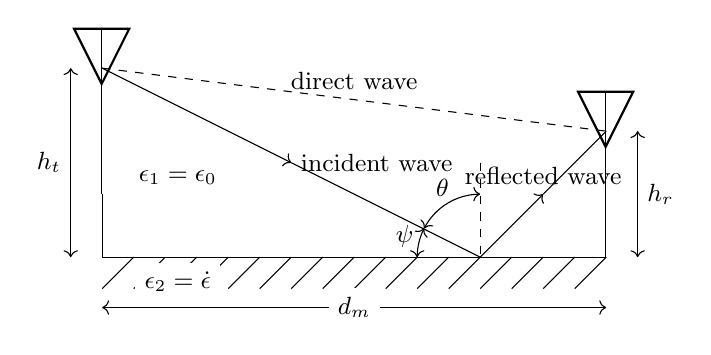
\begin{tikzpicture}[scale=0.8]
		\draw[->] (0,3) --  (3,1.5) node[right]{$\text{incident wave}$}; \draw (3,1.5) -- (6,0); %incident ray
		\draw (1.2,1) node[above]{$\epsilon_1=\epsilon_0$};
		\draw[->] (6,0) -- (7,1) node[above]{$\text{reflected wave}$}; \draw (7,1) -- (8,2); %reflected ray
		\draw[dashed] (6,1.5) -- (6,0); % perpendicular line at reflection point
		\draw (0,0) -- (8,0); % ground plane
	%	\draw (4,0.5) arc (180:220:1cm);
	    \draw[<->] (6,0) ++(180:1) arc(180:153:1); \draw (4.8,0.0) node[above]{$\psi$};
	    \draw[<->] (6,0) ++(153:1) arc(153:90:1); \draw (5.4,0.8) node[above]{$\theta$};
	    \draw (0,-0.5) -- (0.5,0); \draw (0.5,-0.5)--(1,0); \draw (1,-0.5)--(1.5,0); \draw (1.5,-0.5)--(2,0); \draw (2,-0.5)--(2.5,0); \draw (2.5,-0.5)--(3,0); \draw (3,-0.5)--(3.5,0); \draw (3.5,-0.5)--(4,0); \draw (4,-0.5)--(4.5,0); \draw (4.5,-0.5)--(5,0); \draw (5,-0.5)--(5.5,0); \draw (5.5,-0.5)--(6,0); \draw (6,-0.5)--(6.5,0); \draw (6.5,-0.5)--(7,0); \draw (7,-0.5)--(7.5,0); \draw (7.5,-0.5)--(8,0);
	    \draw (1.2,-0.7) node[fill = white, above]{$\epsilon_2=\dot\epsilon$};
	     \draw (0,0) -- (0,1) node[antenna]{};
	     \draw (8,0) node[antenna]{};
%		\draw (0,0) -- (0,3);
%		\draw (8,0) -- (8,2);
	    \draw[dashed] (0,3) --node[above]{$\text{direct wave}$}(8,2) ;
	    \draw[<->] (-0.5,0) --node[left]{$h_t$} (-0.5,3);
	    \draw[<->] (8.5,0) --node[right]{$h_r$} (8.5,2);
	    \draw[<->] (0,-0.8) --node[fill = white,midway]{$d_m$}(8,-0.8) ;
	\end{tikzpicture}
	\caption{Geometry of ground-reflected waves}\label{fig:reflection}
\end{figure}
%Near the earth's surface, the contribution of the surface wave may become important. In this case, the attenuation function is given by
If the surface wave is required, the attenuation function is given by 
\begin{equation}
\label{eq:F}
F = \left\{ 1 - j\sqrt{\pi\nu}e^{-\nu} \left[ \text{erfc}\left(j\sqrt{\nu}\right) \right] \right\},
\end{equation}
where $\text{erfc}$ is the complementary error function. For vertical polarization, the term $\nu$ is given by
\begin{equation}
\label{eq:atten_arg_v}
\nu_v = \dfrac{ -j\omega d_m  }{2\dot\epsilon_rc} \left(1 - \dfrac{\cos^2\psi}{\dot\epsilon_r}\right)
\left[ 1 + \dfrac{\dot\epsilon_r\sin\psi} {\sqrt{ \dot\epsilon_r - \cos^2\psi } } \right]^2,
\end{equation}
while for horizontal polarization it is
\begin{equation}
\label{eq:atten_arg_h}
\nu_h = \dfrac{ -j\omega d_m  }{2c/\dot\epsilon_r} \left(1 - \dfrac{\cos^2\psi}{\dot\epsilon_r}\right)
\left[ 1 + \dfrac{ {\dot\epsilon_r}^{-\frac{1}{2}}\sin\psi } { \sqrt{ \dot\epsilon_r - \cos^2\psi } } \right]^2.
\end{equation}
%In both equations (\ref{eq:atten_arg_v}) and (\ref{eq:atten_arg_h}) $d_m$ is the path length in metres as before.\\

The FWPM results presented here make use of the reflection coefficient approximation which does not compute the surface wave. However, at the expense of longer simulation runtime the model can be set to utilize the full Sommerfeld formulation which will incorporate the contribution of the surface wave to the received field. %It must be noted that the simulation runtime doubles when the Sommerfeld equations are . %Surface wave contributions are neglected here as they have been found to be insignificant in the configuration of interest.
%
\subsection{Simulation Setup and Validation}
Simulated path loss was computed via S-Parameters as
\begin{equation}
PL_s = 10\log \left|\dfrac{1}{ S_{21}{'}}\right|^2 + 2G,
\end{equation}
where $\left|S_{21}{'}\right|^2 \equiv \text{power received}/\text{power radiated}$ is the transmission coefficient corrected for mismatch and $G$ is the gain of transmitter and receiver in \SI{}{dBi}. To ensure that the FEKO model was correctly configured, a comparison was made to theory (equation (\ref{eqn:FSL2})). As can be seen from the sample result in Fig \ref{fig:sim_fsl}, the simulated prediction is in good agreement with the theoretical formulation of the Friis transmission equation. This is quite a remarkable result that highlights the power of a full-wave simulation. % What is the power of a full-wave simulation??
\begin{figure}
	\centering
	{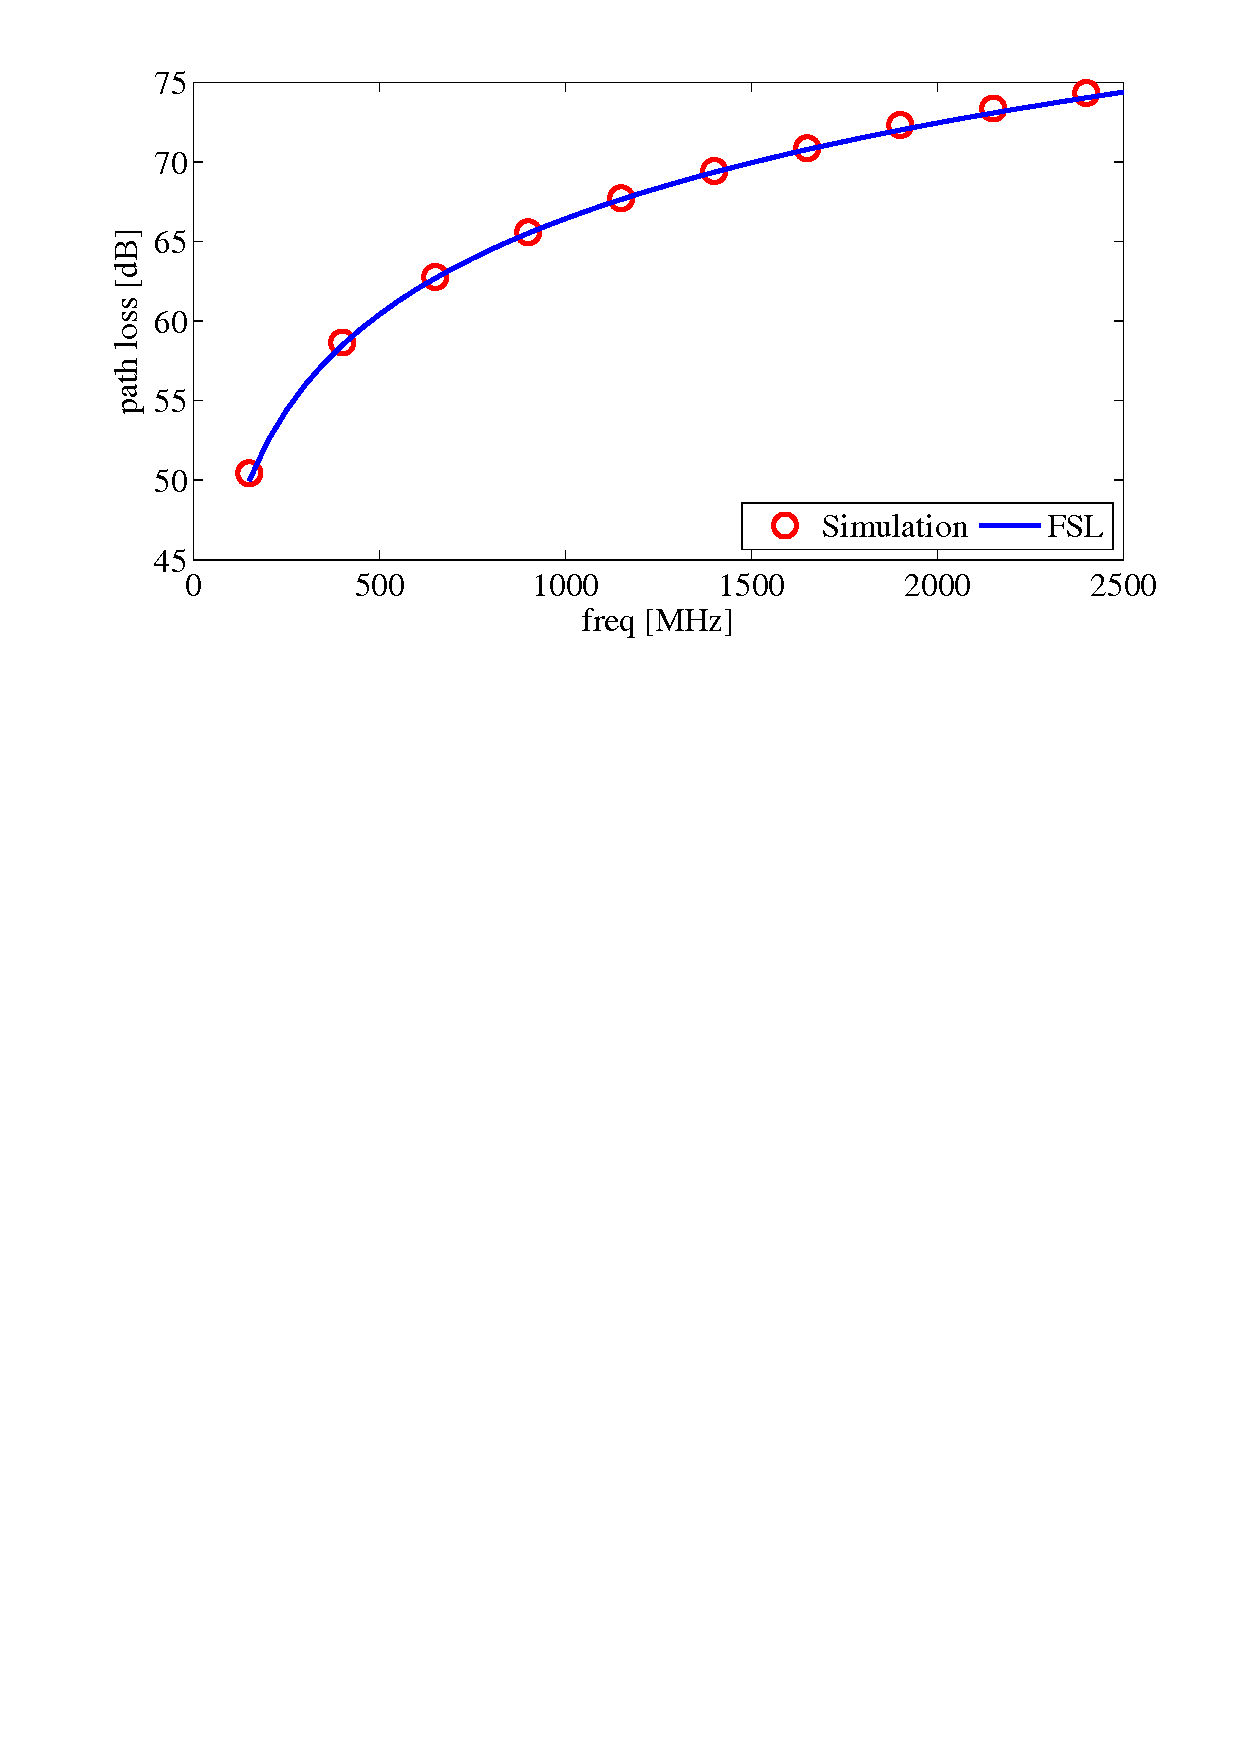
\includegraphics[width=\linewidth]{path_loss_verification_50m}}
	\caption{Free space path loss predictions at a T-R distance of \SI{50}{m}}
	\label{fig:sim_fsl}
\end{figure} 
%
\section{Comparison of FWPM Predictions to Measured Data}\label{Comparison of FWPM Predictions to Measured Data}
%
\subsection{Measurements in a Controlled Environment}
Path loss results can change quite dramatically when transmission takes place in the vicinity of the ground such as when transceiver heights are low. In a `simple' scenario involving a flat ground, the key issue for the FWPM is with regard to the value of $\dot\epsilon_r$ in modelling the electrical characteristics of the earth. Conditions of the soil change with seasonal variations so that the actual electrical parameters will seldom be known. A working approximation must thus be established. To do this, predictions from three types of simulated ground were compared to measured data that was obtained at a field akin to an open area test site. A summary of the equipment used is presented in Table~\ref{tb:specs1}.
%
\begin{table} %[!h]
	\renewcommand{\arraystretch}{1.5}
		\caption{Equipment used for Verification Measurements}
		\label{tb:specs1}
		\centering
%		\setlength{\tabcolsep}{20pt}
		\begin{tabular}{lccc}\toprule
			\multicolumn{4}{c}{AnaPico APSIN\num{6010} DC Generator}\\ \midrule
			\multicolumn{2}{l|}{output power (used)} & \multicolumn{2}{c}{\SI{-20}{dBm}} \\
			\multicolumn{2}{l|}{frequency range} & \multicolumn{2}{c}{\SI{0.009} - \SI{6100}{MHz}} \\ \midrule
			\multicolumn{4}{c}{PCB-LPDA (transmitter and receiver)}\\ \midrule
			\multicolumn{2}{l|}{average gain} & \multicolumn{2}{c}{\SI{5}{dBi}}\\
			\multicolumn{2}{l|}{frequency range}  & \multicolumn{2}{c}{\SI{400} - \SI{6000}{MHz}} \\ \midrule
			\multicolumn{4}{c}{FSH4 Handheld Spectrum Analyser (SA)}\\ \midrule
			\multicolumn{2}{l|}{sensitivity} & \multicolumn{2}{c}{\SI{-141}{dBm}}\\
			\multicolumn{2}{l|}{frequency range} & \multicolumn{2}{c}{\SI{0.009} - \SI{3600}{MHz}} \\ \bottomrule			
		\end{tabular}
\end{table}
%

A PCB-LPDA was connected to the Anapico DC signal generator to form the transmitting unit while the receiver unit comprised a similar PCB-LPDA and the FSH4 handheld spectrum analyser. With the transmitting antenna fixed at a height of \SI{5}{m} and the receiving antenna at \SI{2}{m}, the maximum received power was recorded at five distances between \SI{20}{} and \SI{200}{m}. Some results are shown in Fig \ref{fig:pl_control} while statistical analysis of the predictions is presented in Table \ref{tb:stats1}. Although all three FWPM simulations yield very good predictions, based on the root mean square errors the best approximation to the measurement scenario is the medium dry ground setup. More significantly, it can be seen that the question of path loss below \SI{1}{km} is not trivially equivalent to free space loss as often presumed. The maximum residual for FSL predictions lies \num{4.65} standard deviations from the mean but is \num{3.68} for the worst performing FWPM prediction. Evidently, free space path loss exhibits a significant deviation which can be costly where accuracy is required.
%
\begin{table*}[!ht]
	\caption{Mean Prediction Error and RMSE Analysis for the FWPM Validation}
	\label{tb:stats1}
	\centering
	\renewcommand{\arraystretch}{1.3}
	\setlength{\tabcolsep}{3pt}
	\begin{tabular*}{\linewidth}{ @{\extracolsep{\fill}} l*{16}c @{}}\toprule
		$d_m$ & \multicolumn{4}{c}{Prediction Error, $\bar\varepsilon$ [\SI{}{dB}]} & \multicolumn{4}{c}{Max Residual, $\varepsilon_{\text{max}}$ [\SI{}{dB}]} & \multicolumn{4}{c}{Standard Dev, $\sigma_{\bar\varepsilon}$ [\SI{}{dB}]} & \multicolumn{4}{c}{RMSE [\SI{}{dB}]}\\ \cmidrule{1-1} \cmidrule{2-5} \cmidrule{6-9} \cmidrule{10-13} \cmidrule{14-17}%\hline\hline
		$[\SI{}{m}]$ & dry & med & wet & FSL & dry & med & wet & FSL & dry & med & wet & FSL & dry & med & wet & FSL\\
		 \cmidrule{1-1} \cmidrule{2-5} \cmidrule{6-9} \cmidrule{10-13} \cmidrule{14-17}
		20   & 1.96 & 2.36 & 2.65 & 8.41 &{} 8.44  & 7.42  & 8.34  & 13.87 &{} 2.85 & 2.19 & 2.22 & 2.33 &{} 3.46 & 3.22 & 3.45 & 8.73\\
		50   & 2.50 & 2.92 & 3.25 & 8.35 &{} 16.05 & 14.76 & 14.06 & 19.70 &{} 3.92 & 3.71 & 3.92 & 4.44 &{} 4.65 & 4.71 & 5.09 & 9.45\\
		100  & 2.54 & 2.69 & 2.82 & 6.86 &{} 13.40 & 12.67 & 12.23 & 18.13 &{} 5.54 & 4.58 & 4.08 & 3.73 &{} 6.09 & 5.31 & 4.96 & 7.81\\
		150  & 0.91 & 1.21 & 1.42 & 5.74 &{} 16.33 & 16.18 & 16.17 & 23.21 &{} 4.30 & 3.84 & 3.71 & 5.03 &{} 4.39 & 4.02 & 3.96 & 7.63\\
		200  & 2.01 & 1.98 & 1.97 & 4.54 &{} 8.00  & 8.02  & 8.04  & 11.21 &{} 1.87 & 1.97 & 2.06 & 2.97 &{} 2.75 & 2.78 & 2.85 & 5.43\\ \cmidrule{1-1} \cmidrule{2-5} \cmidrule{6-9} \cmidrule{10-13} \cmidrule{14-17}
		mean & 1.99 & 2.23 & 2.42 & 6.78 &{} 12.44 & 11.81 & 11.77 & 17.22 &{} 3.70 & 3.26 & 3.20 & 3.70 &{} 4.27 & 4.01 & 4.06 & 7.81\\ \bottomrule
	\end{tabular*}
\end{table*}
%
\begin{figure*}[!ht]
	\centering
	\subfloat[]{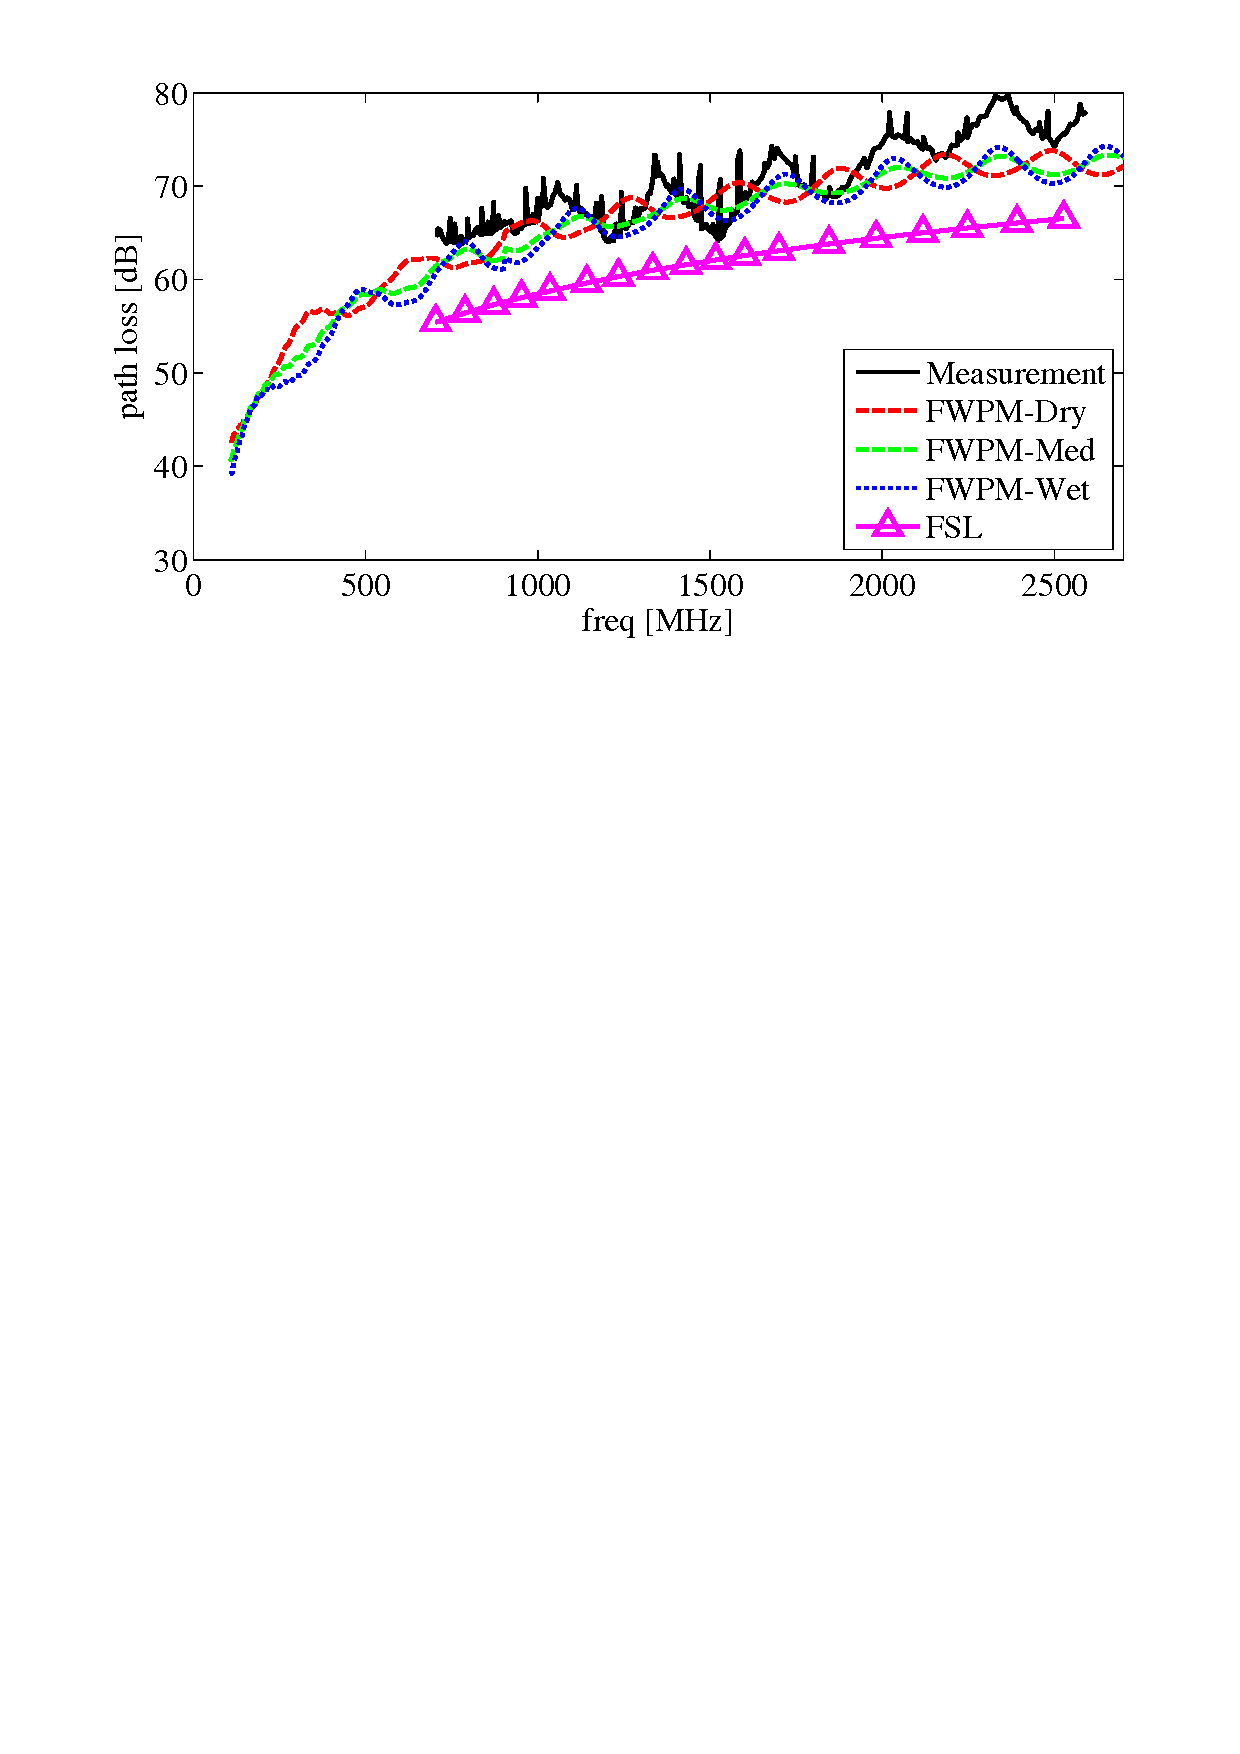
\includegraphics[width=0.32\linewidth]{hockey-20m}%
		\label{fig:pl20}}%
	\hfil
	\subfloat[]{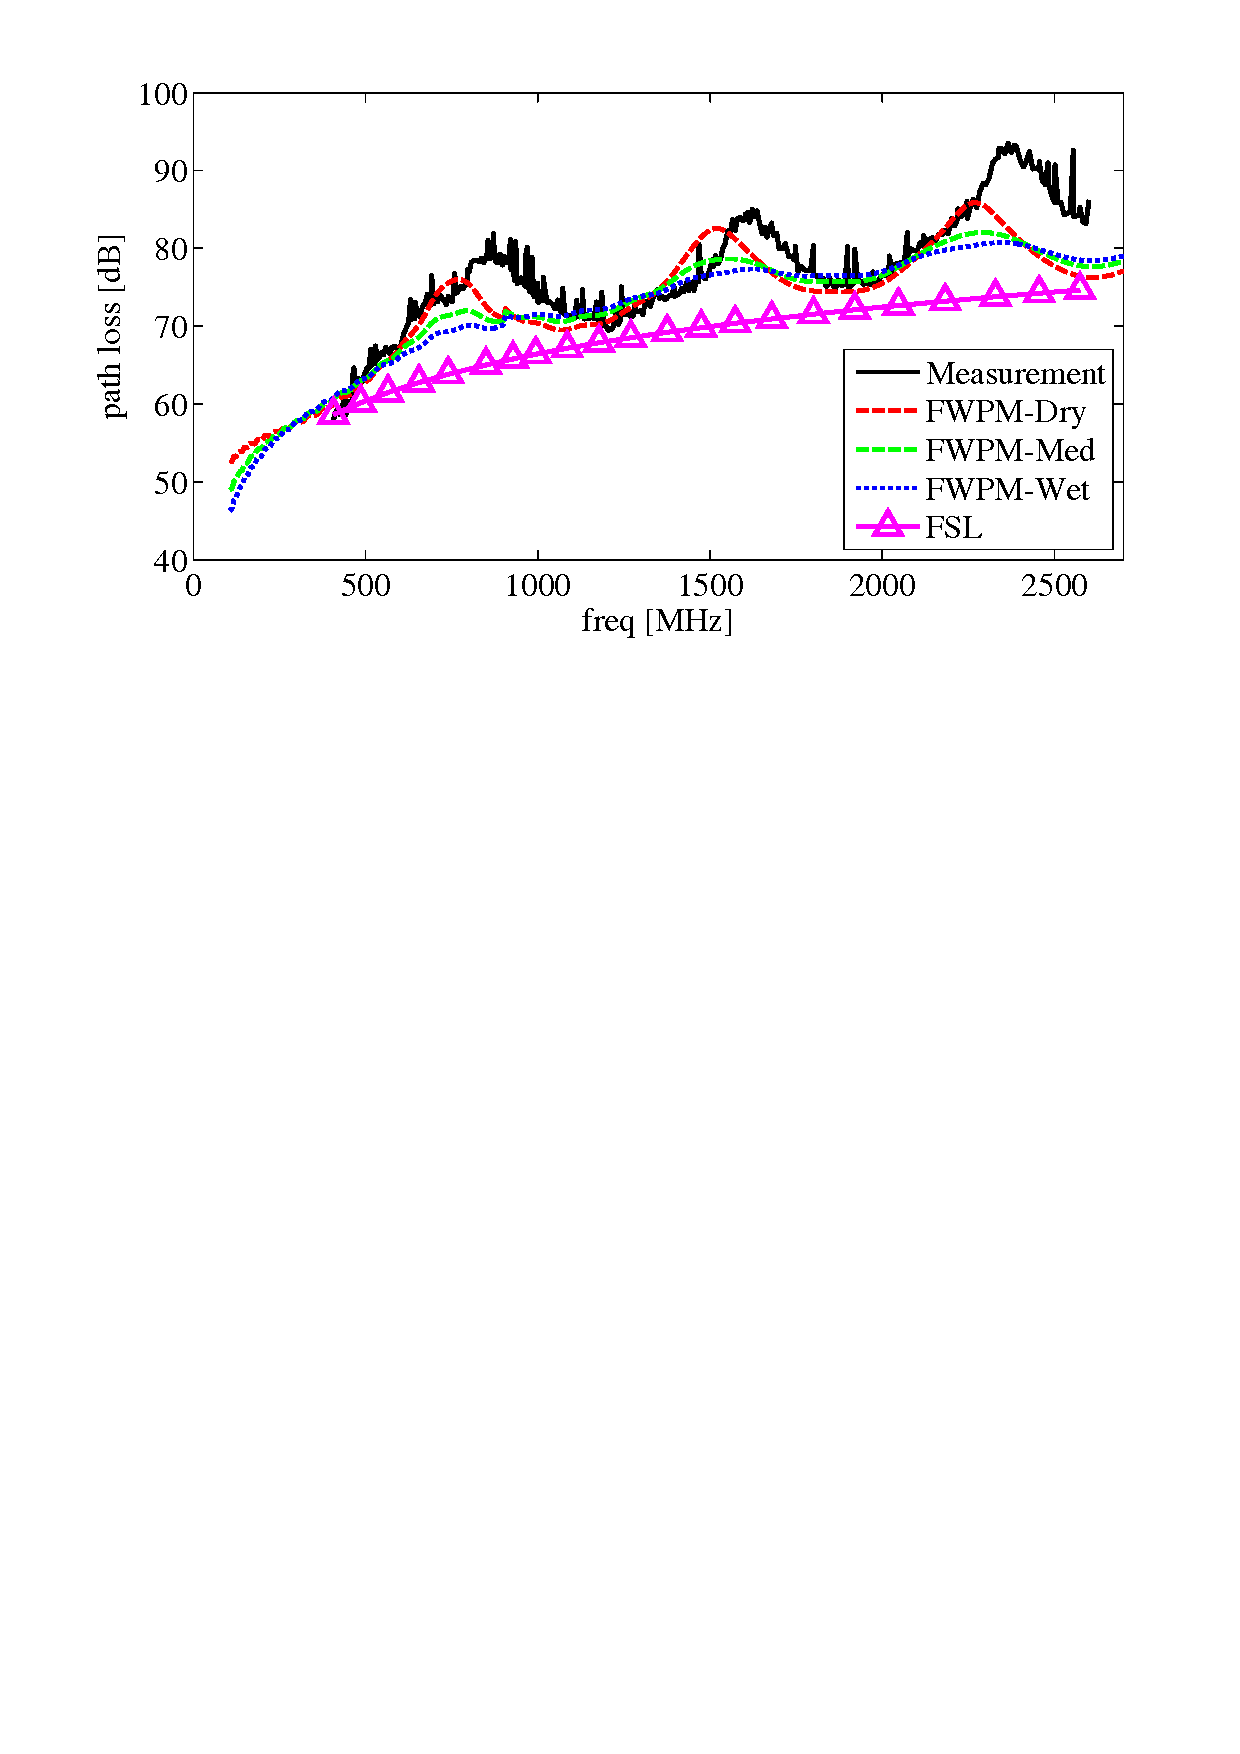
\includegraphics[width=0.32\linewidth]{hockey-50m.pdf}%
		\label{fig:pl50}}%
	\hfil
	\subfloat[]{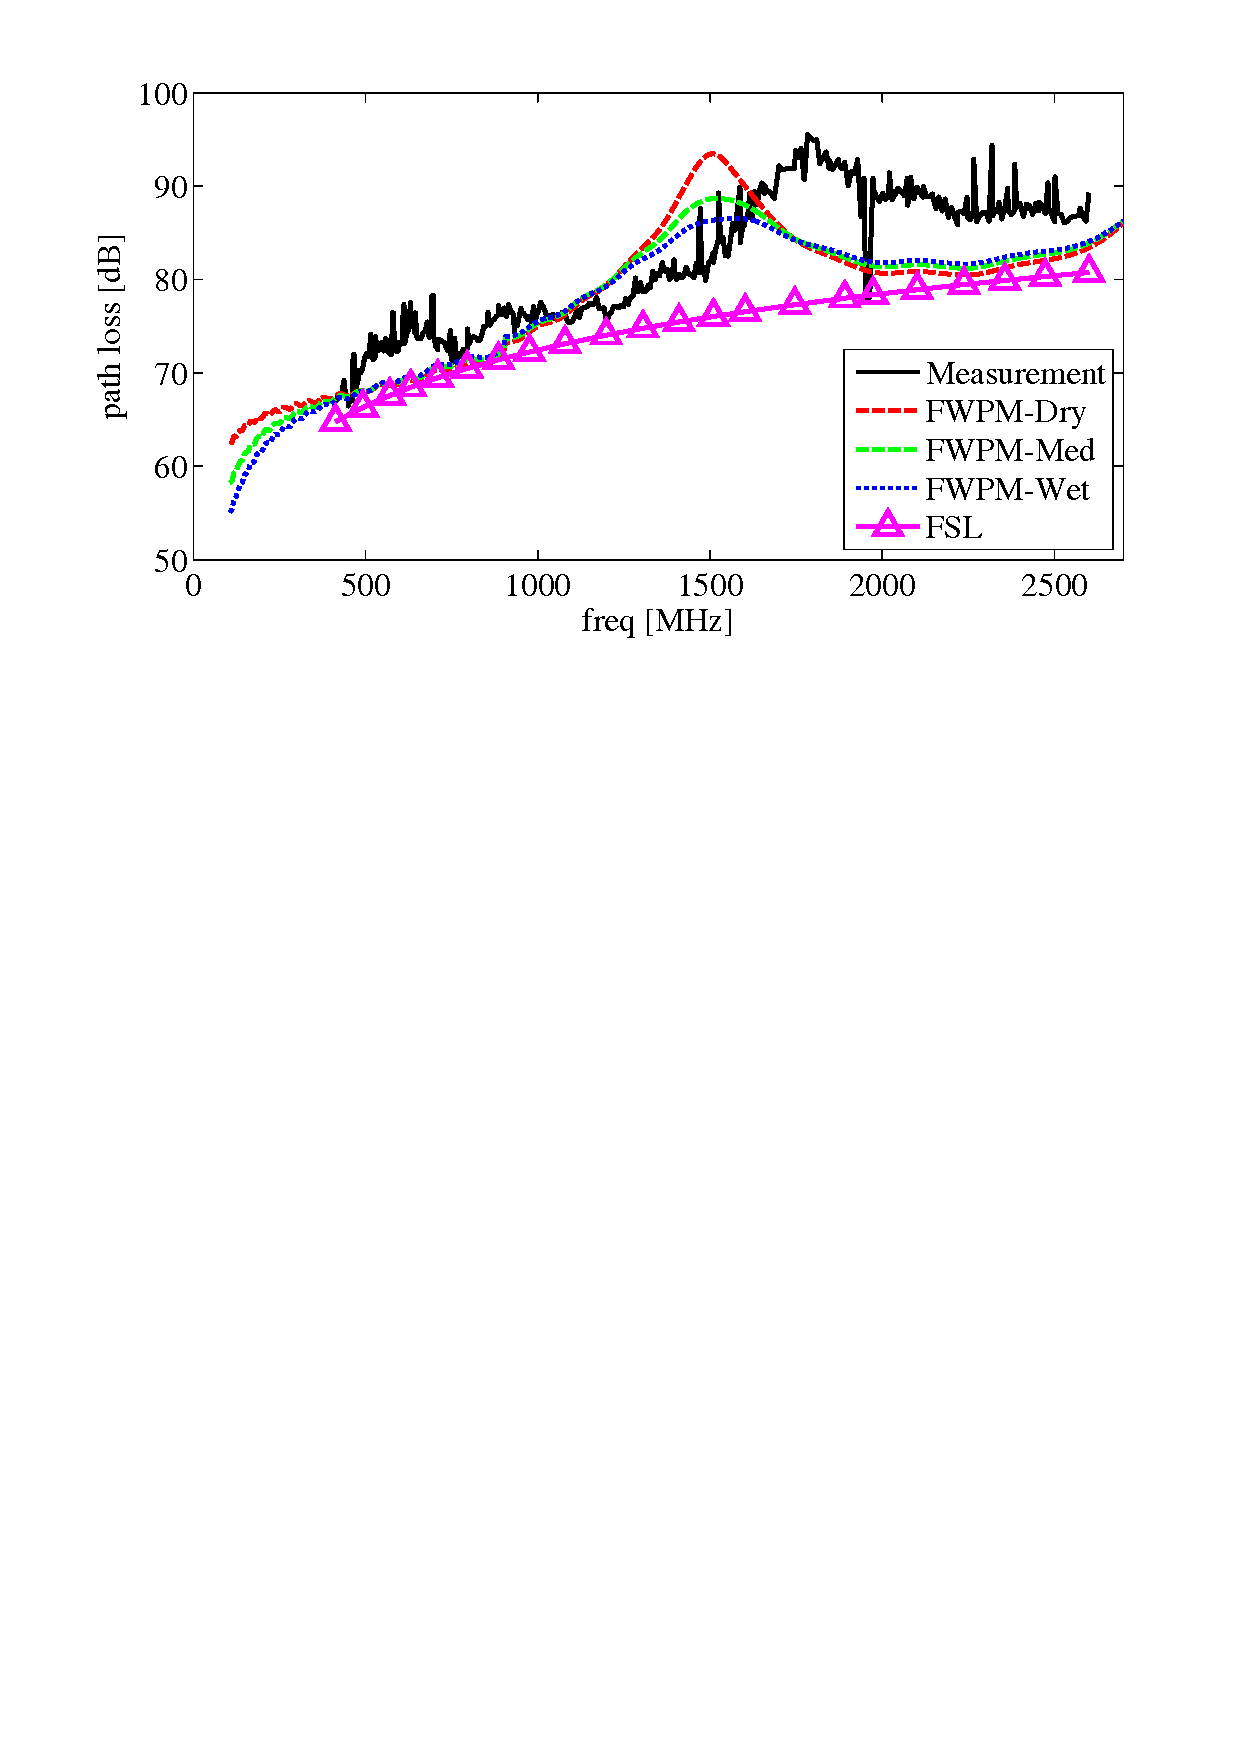
\includegraphics[width=0.32\linewidth]{hockey-100m.pdf}%
		\label{fig:pl100}}
	\caption{Open area measurements and predicted path loss at T-R separations of \protect\subref{fig:pl20} \SI{20}{m}, \protect\subref{fig:pl50} \SI{50}{m} and \protect\subref{fig:pl100} \SI{100}{m}. In all cases $h_t = \SI{5}{m}$ and $h_r = \SI{2}{m}$}
	\label{fig:pl_control}
\end{figure*}
%
\subsection{Case Study: Field Measurements in the Karoo}
The Karoo is a semi-desert region in South Africa's Northern Cape Province and is home to MeerKAT -- a Square Kilometre Array Telescope precursor. Propagation modelling has a vital role to play in the furtherance of good EMC and spectrum management practices wherein predictions form part of the basis on which RFI threshold levels are determined. The need for accuracy cannot therefore be overstated.\\
Recently, a comparative study used data obtained at the MeerKAT site to examine the efficacy of ITU-R P.\num{1546} and ITM models for path loss predictions at shorter path lengths and lower transceiver heights than originally intended \cite{Phiri}. While acceptable error margins were reported, it is desirable to achieve higher accuracy and synthesize a site-specific model to aid electromagnetic characterisation of the MeerKAT environment.

Karoo data analysed here is the same dataset as in \cite{Phiri}. Equipment used during the measurement campaign included a CPS1 pulse generator, LPDA (R\&S HL033) and a horn antenna (EM-7020) at the transmitting end. On the receiving end, two LPDA's (R\&S HL023 and a custom-built PCB-LPDA) were deployed in conjunction with a real-time analyser (RTA). Use of the pulser and RTA made broadband time-domain recordings possible, speeding up the survey time significantly. Measurements were recorded for vertical polarization transmissions at five T-R separation distances between \SI{50}{} and \SI{3600}{m} for transmitter heights of \SI{5}{} and \SI{7.5}{m}. With free space loss as a reference, measured and predicted path loss curves are shown in Figs \ref{fig:karoo_LL} and \ref{fig:karoo_LH}. % while the statistical analysis on the FWPM predictions is shown in Table \ref{tb:stats2}. %as a first step in the realization of a site-specific model.
%
%The uncertainty due to unknown transmitter gain was removed in this dataset. Nonetheless, it was observed that the data oddly deviated from predictions at the lower ($<\SI{0.5}{GHz}$) rather than higher frequencies. These deviations were attributed to increased interactions with the terrain in respect of Fresnel clearance zones \cite{MESA}.

Statistical analysis on the FWPM predictions is provided in Table \ref{tb:stats2}. The row designated mean 1 is the average value corresponding to path lengths below \SI{1}{km} while mean 2 is the average across all path lengths. Predictions of the free space loss (FSL) model are acceptable in respect of the \SI{10}{} -- \SI{15}{dB} RMSE allowance for rural areas. Under a kilometre, \SI{6.70}{} and \SI{8.06}{dB} were obtained for the two respective cases, while \SI{11.22}{} and \SI{11.53}{dB} were obtained overall. However, if the individual path is considered, FSL predictions fall outside the acceptable margin above \SI{1}{km}. In contrast, \SI{3.08}{} and \SI{3.57}{dB} RMSE is obtained overall for the FWPM predictions.\\
In terms of relative error, the FWPM yields a fractional error that is less than \num{0.05} which is equivalent to a confidence level (accuracy) greater than \SI{95}{\%} which is desired. FSL modelling fails this test with \SI{93}{\%} accuracy at best. Correlation is strong for both models particularly at short ranges. Slightly more linear closeness is seen in the FSL model in the second configuration ($h_t=\SI{7.5}{m}$) but overall the FWPM performs better with correlation coefficients of \num{0.729} and \num{0.795} versus \num{0.633} and \num{0.757} for FSL.

Electrical parameters corresponding to wet ground were found to provide the best fit to Karoo data. Assuming that the predominant source of attenuation is ground loss, this would suggest that the relative permittivity of Karoo soil is on the order of \num{32}. This value stands in stark contrast to attempts that have been made at extracting the complex permittivity of Karoo soil such as in \cite{Braam2011} where a value of \num{3.8} (typical for dry ground) is reported for the S and X bands. However, this is presently not problematic since this work does not attempt to determine the value of $\epsilon_r$ but focuses on accounting for its effects with respect to obtaining the best predictions. It is probable that the shallow aquifers of the Karoo result in a higher soil moisture content than typical arid regions.\\ %Moreover, this discrepancy might be due to differences in moisture content at the time of the respective measurements. 
Determining the exact values of complex permittivity is desirable but highly challenging particularly since properties such as compactness and moisture content of the soil change as soon as it has been removed from its locale. Hence, for propagation modelling, finding the best fit using existing data may be the most practical approach.
%
\begin{figure*}[!ht]
	\centering
	\subfloat[]{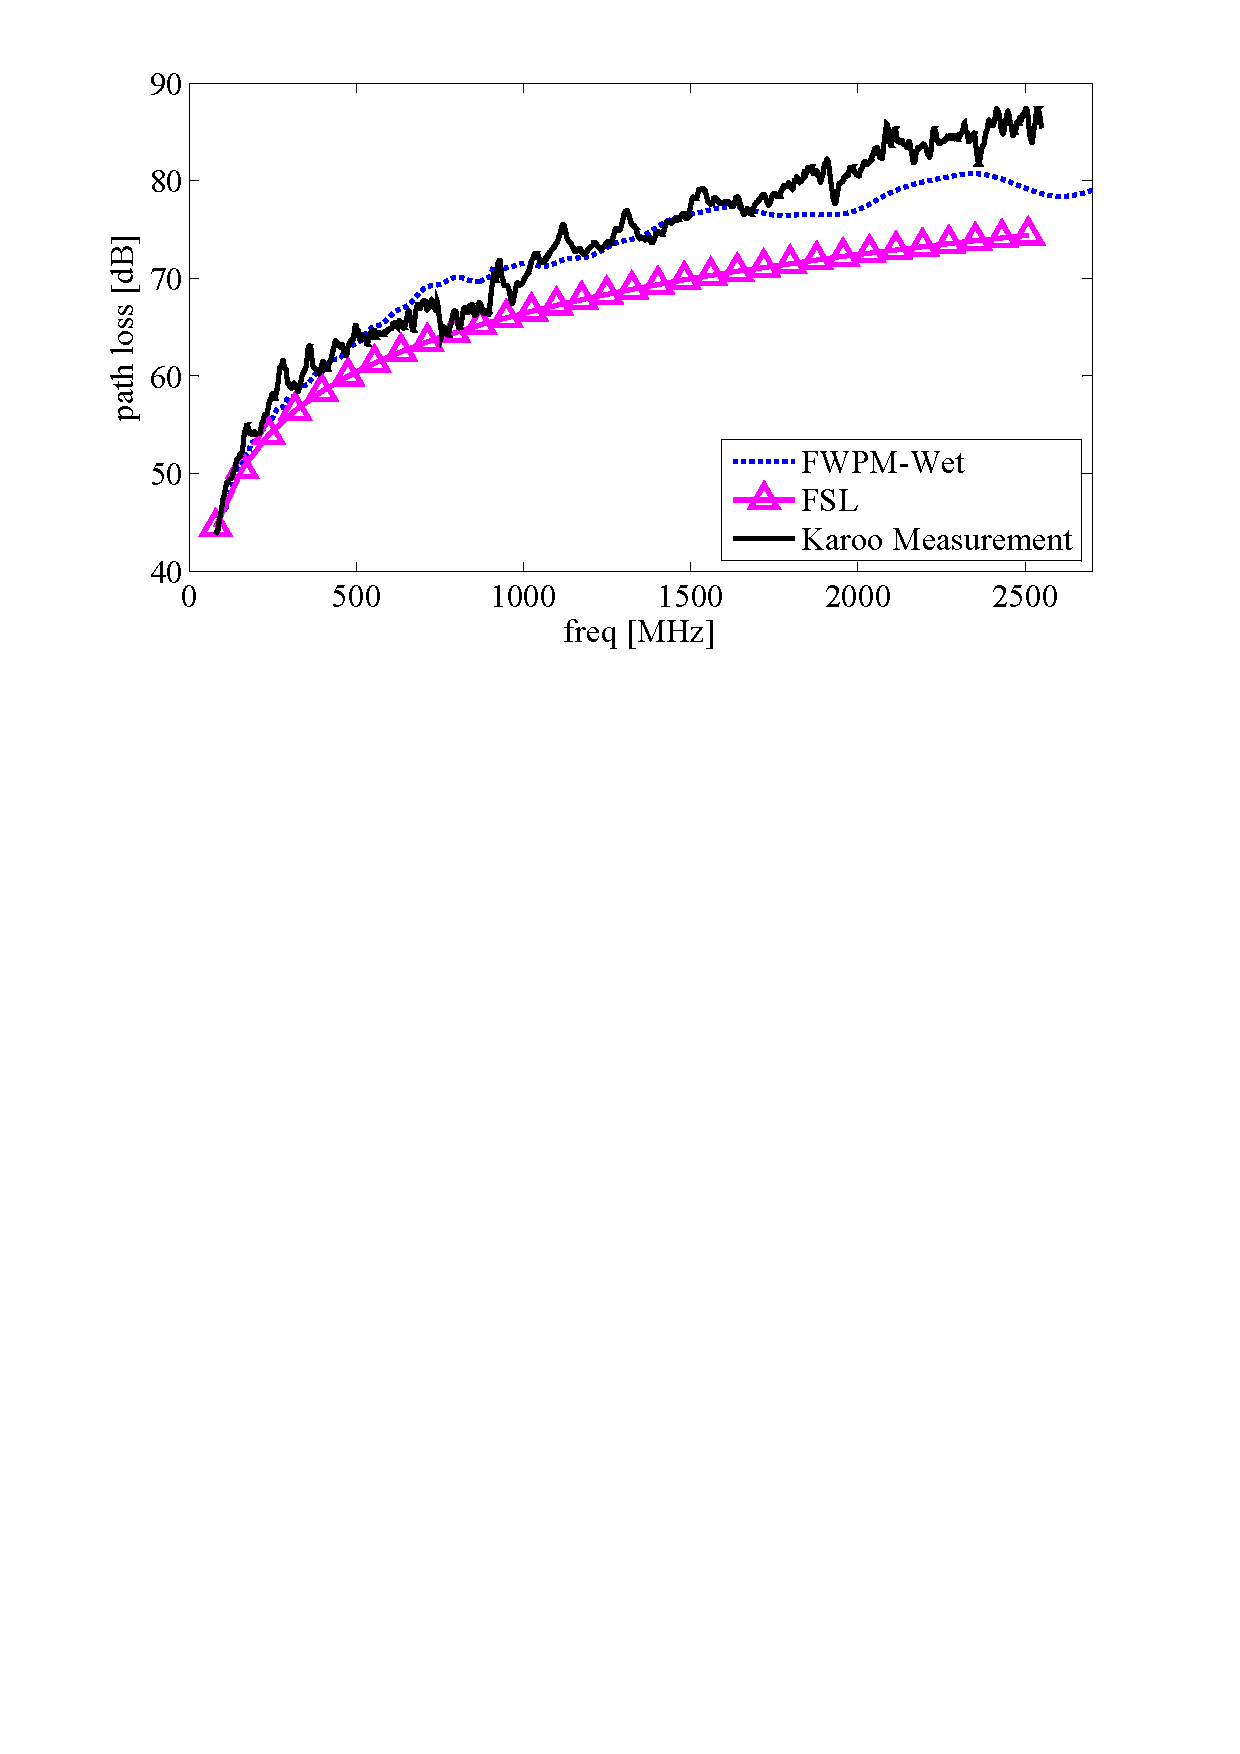
\includegraphics[width=0.32\linewidth]{Karoo_LL_50m}%
	\label{fig:karoo_LL_50m}}%
%	\caption{Measured and predicted path loss in the Karoo: T-R separation of \SI{200}{m}}
    \hfil
	\subfloat[]{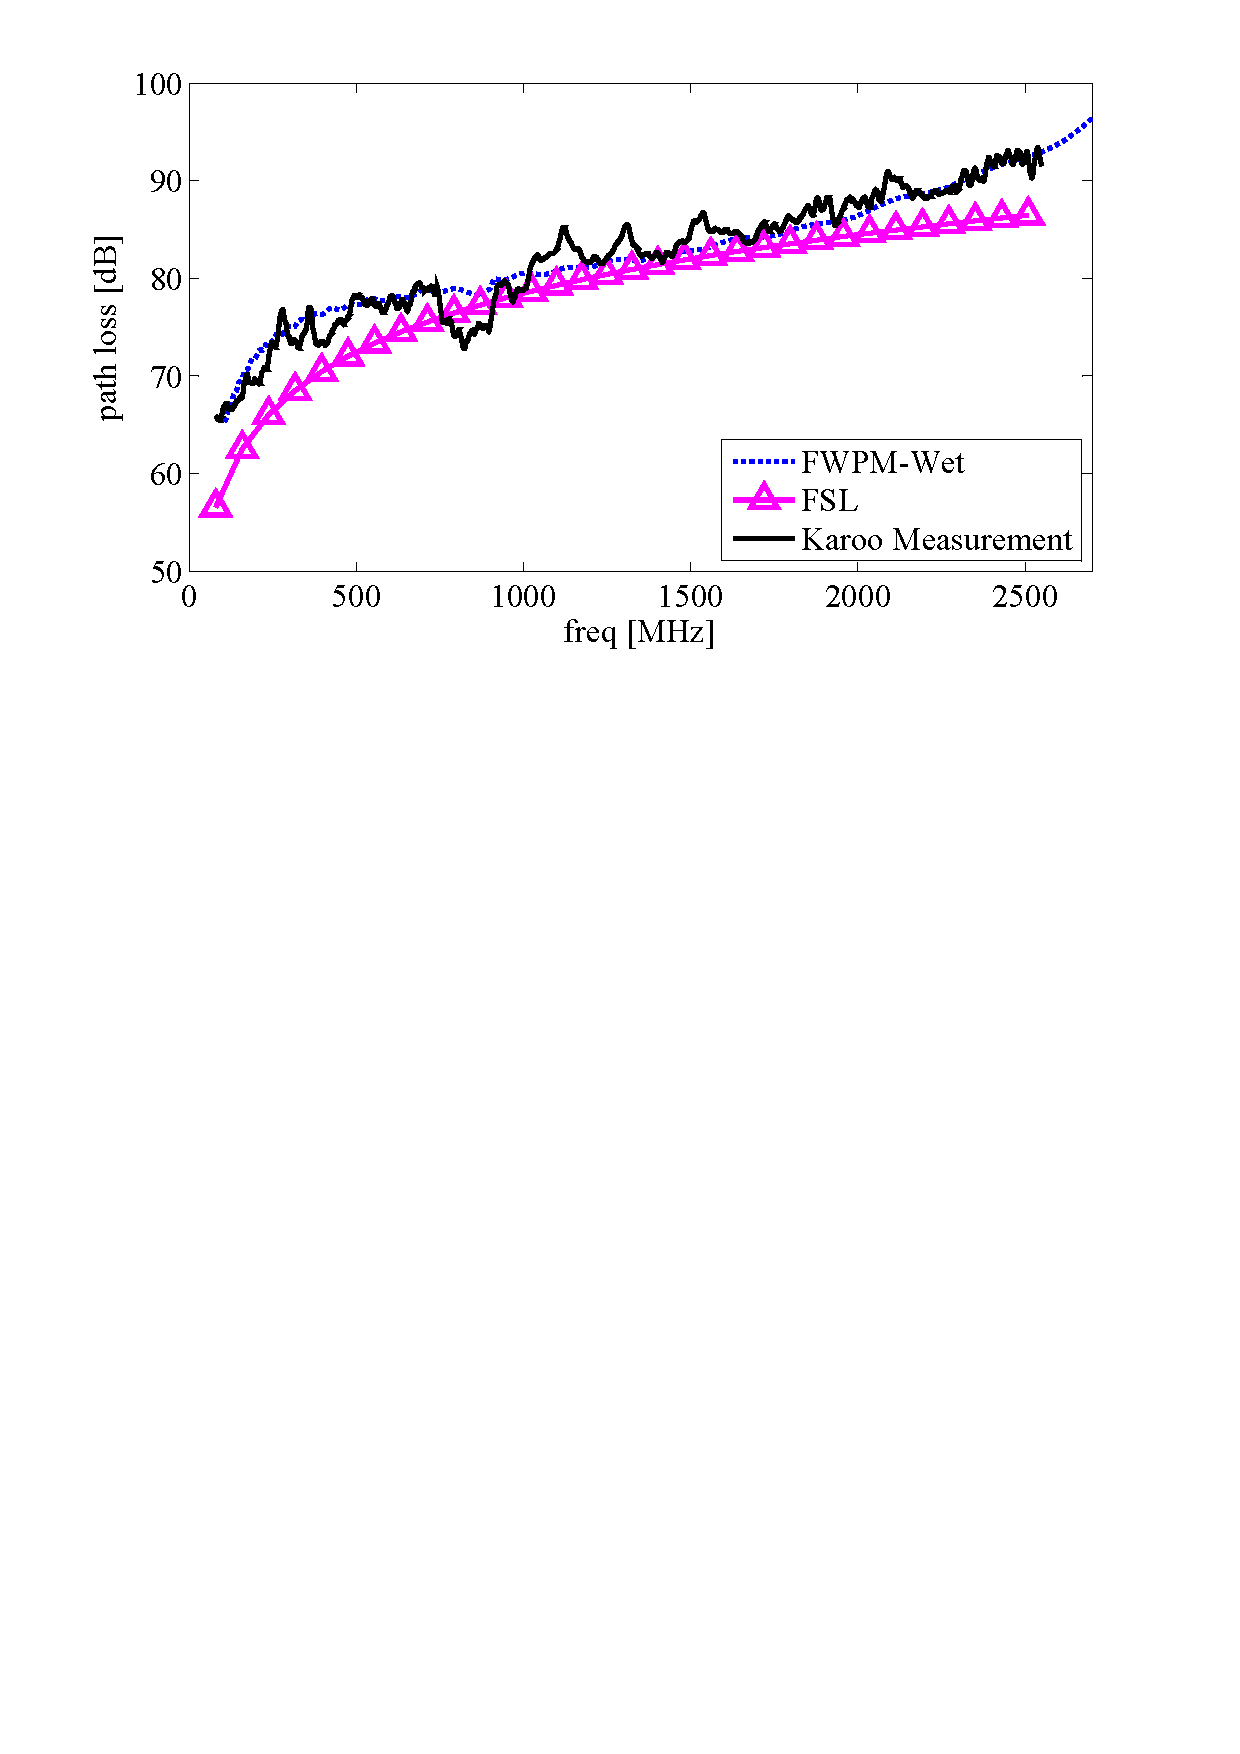
\includegraphics[width=0.32\linewidth]{Karoo_LL_200m}%
	\label{fig:karoo_LL_200m}}%
%	\caption{Measured and predicted path loss in the Karoo: T-R separation of \SI{700}{m}}
    \hfil
	\subfloat[]{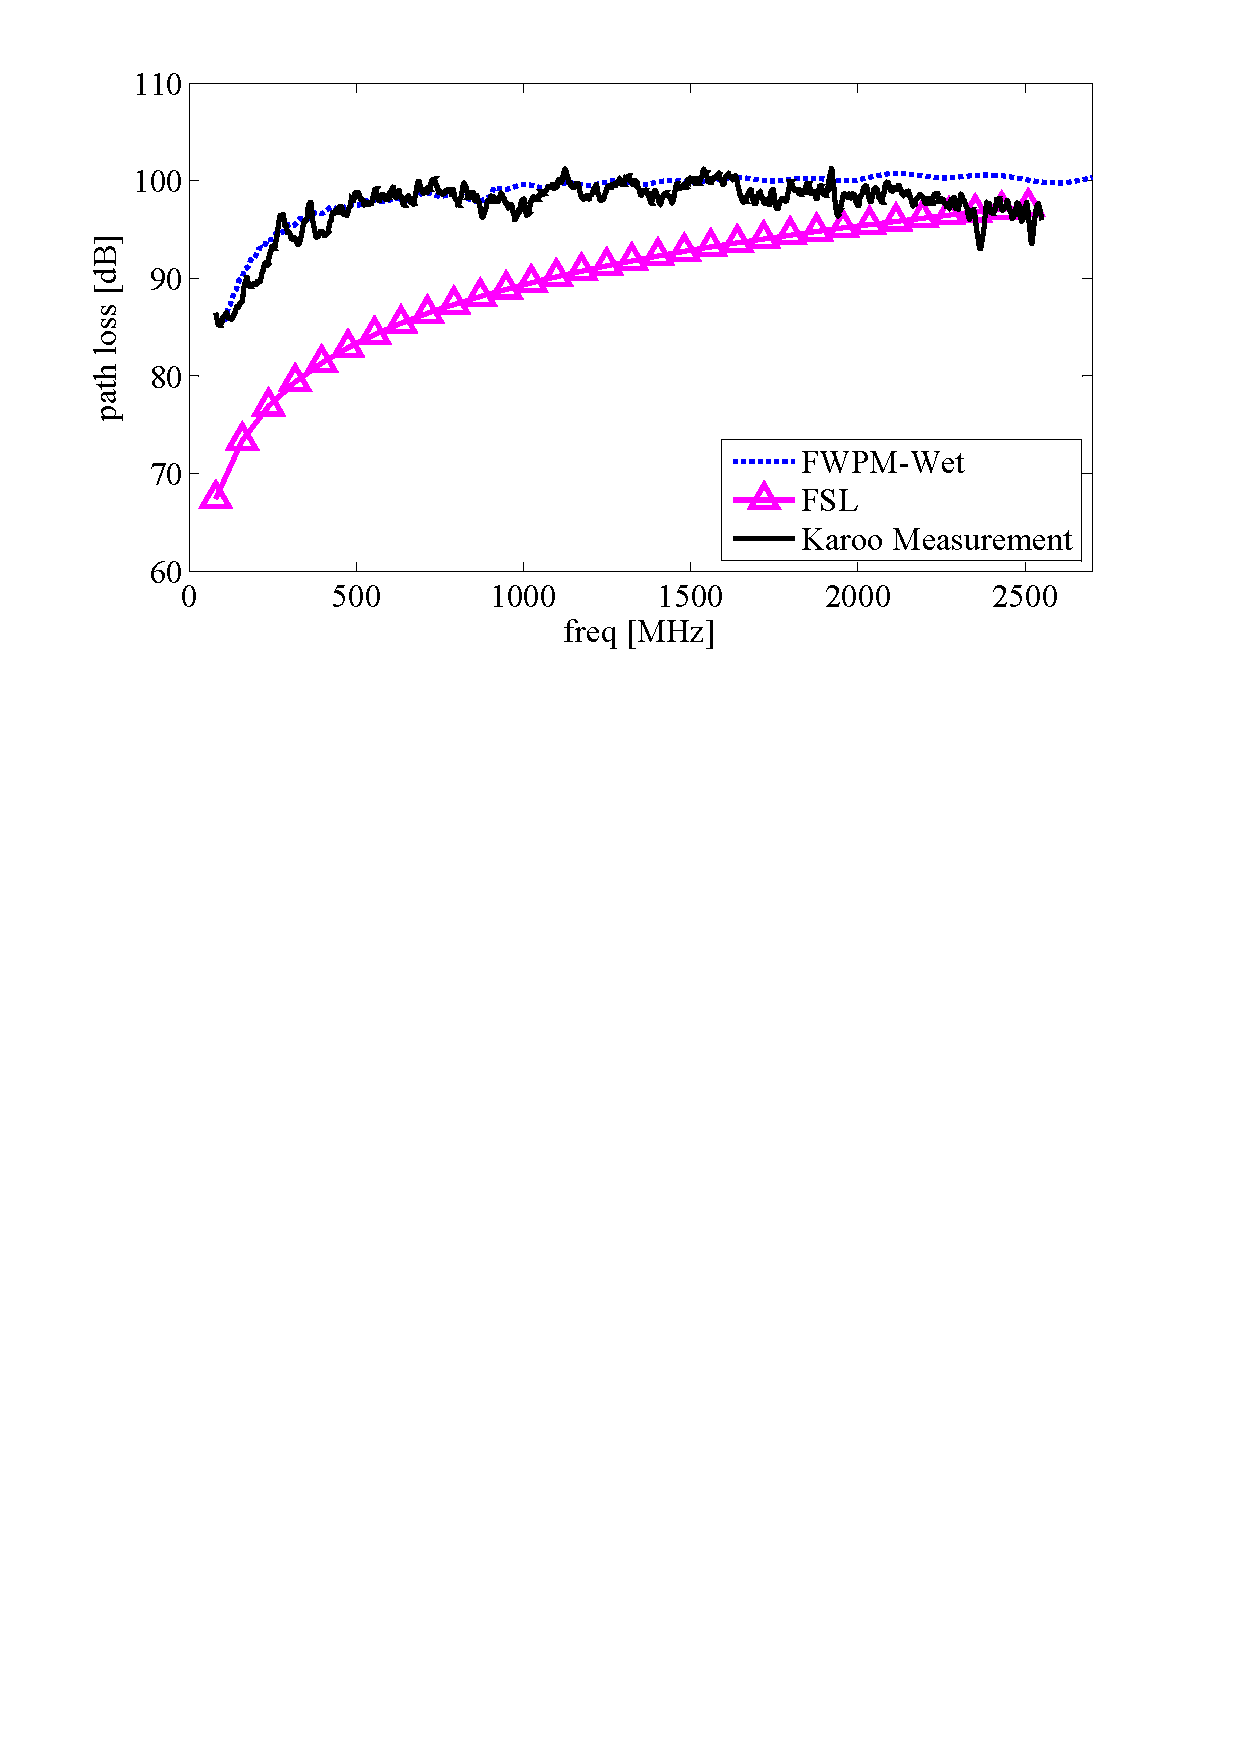
\includegraphics[width=0.32\linewidth]{Karoo_LL_700m}%
	\label{fig:karoo_LL_700m}}%
	\caption{Measured and predicted path loss in the Karoo: $h_t = \SI{5}{m}$, $h_r = \SI{2}{m}$ at T-R separations of \protect\subref{fig:karoo_LL_50m} \SI{50}{m}, \protect\subref{fig:karoo_LL_200m} \SI{200}{m} and \protect\subref{fig:karoo_LL_700m} \SI{700}{m}}%
	\label{fig:karoo_LL}%
\end{figure*}%
%  
\begin{figure*}[!ht]
	\centering
	\subfloat[]{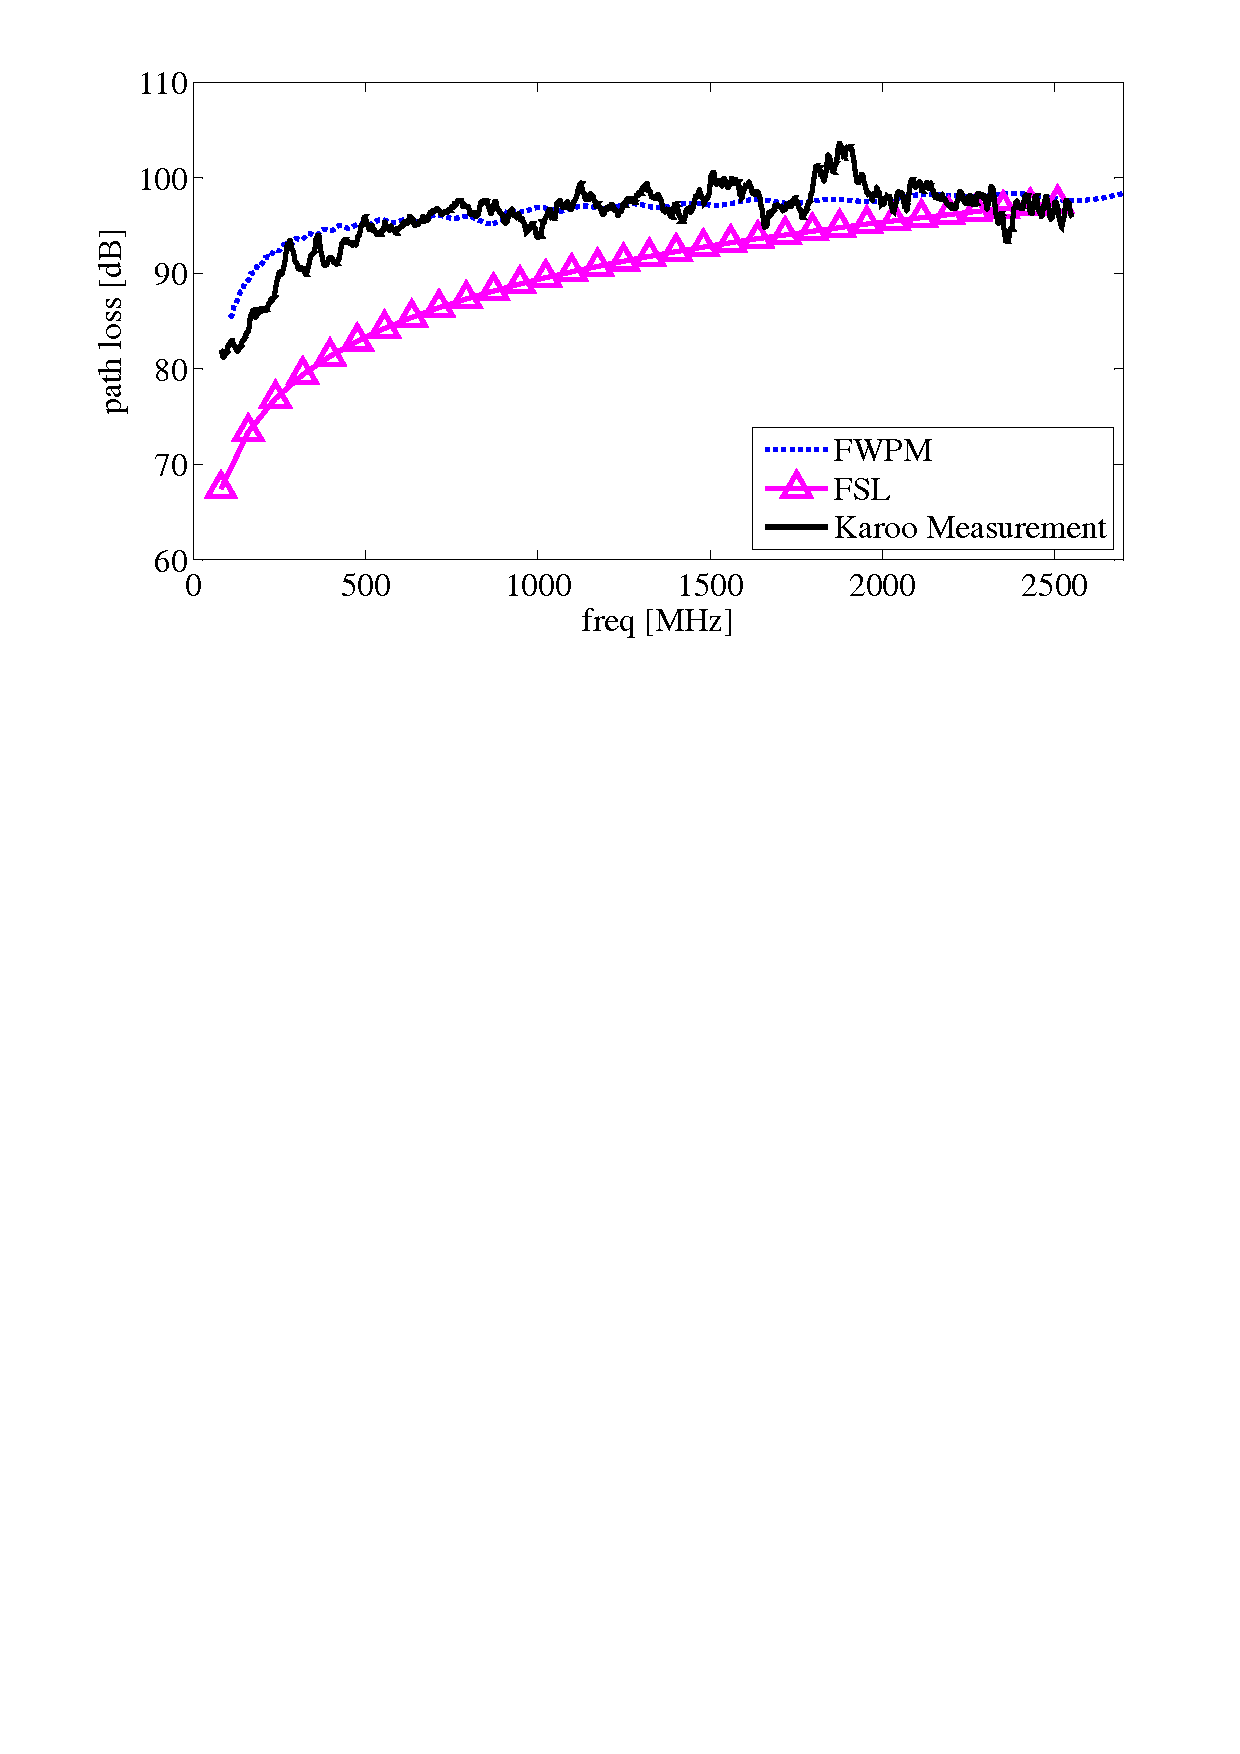
\includegraphics[width=0.32\linewidth]{Karoo_LH_700m}%
	\label{fig:karoo_LH_700m}}%
    \hfil
	\subfloat[]{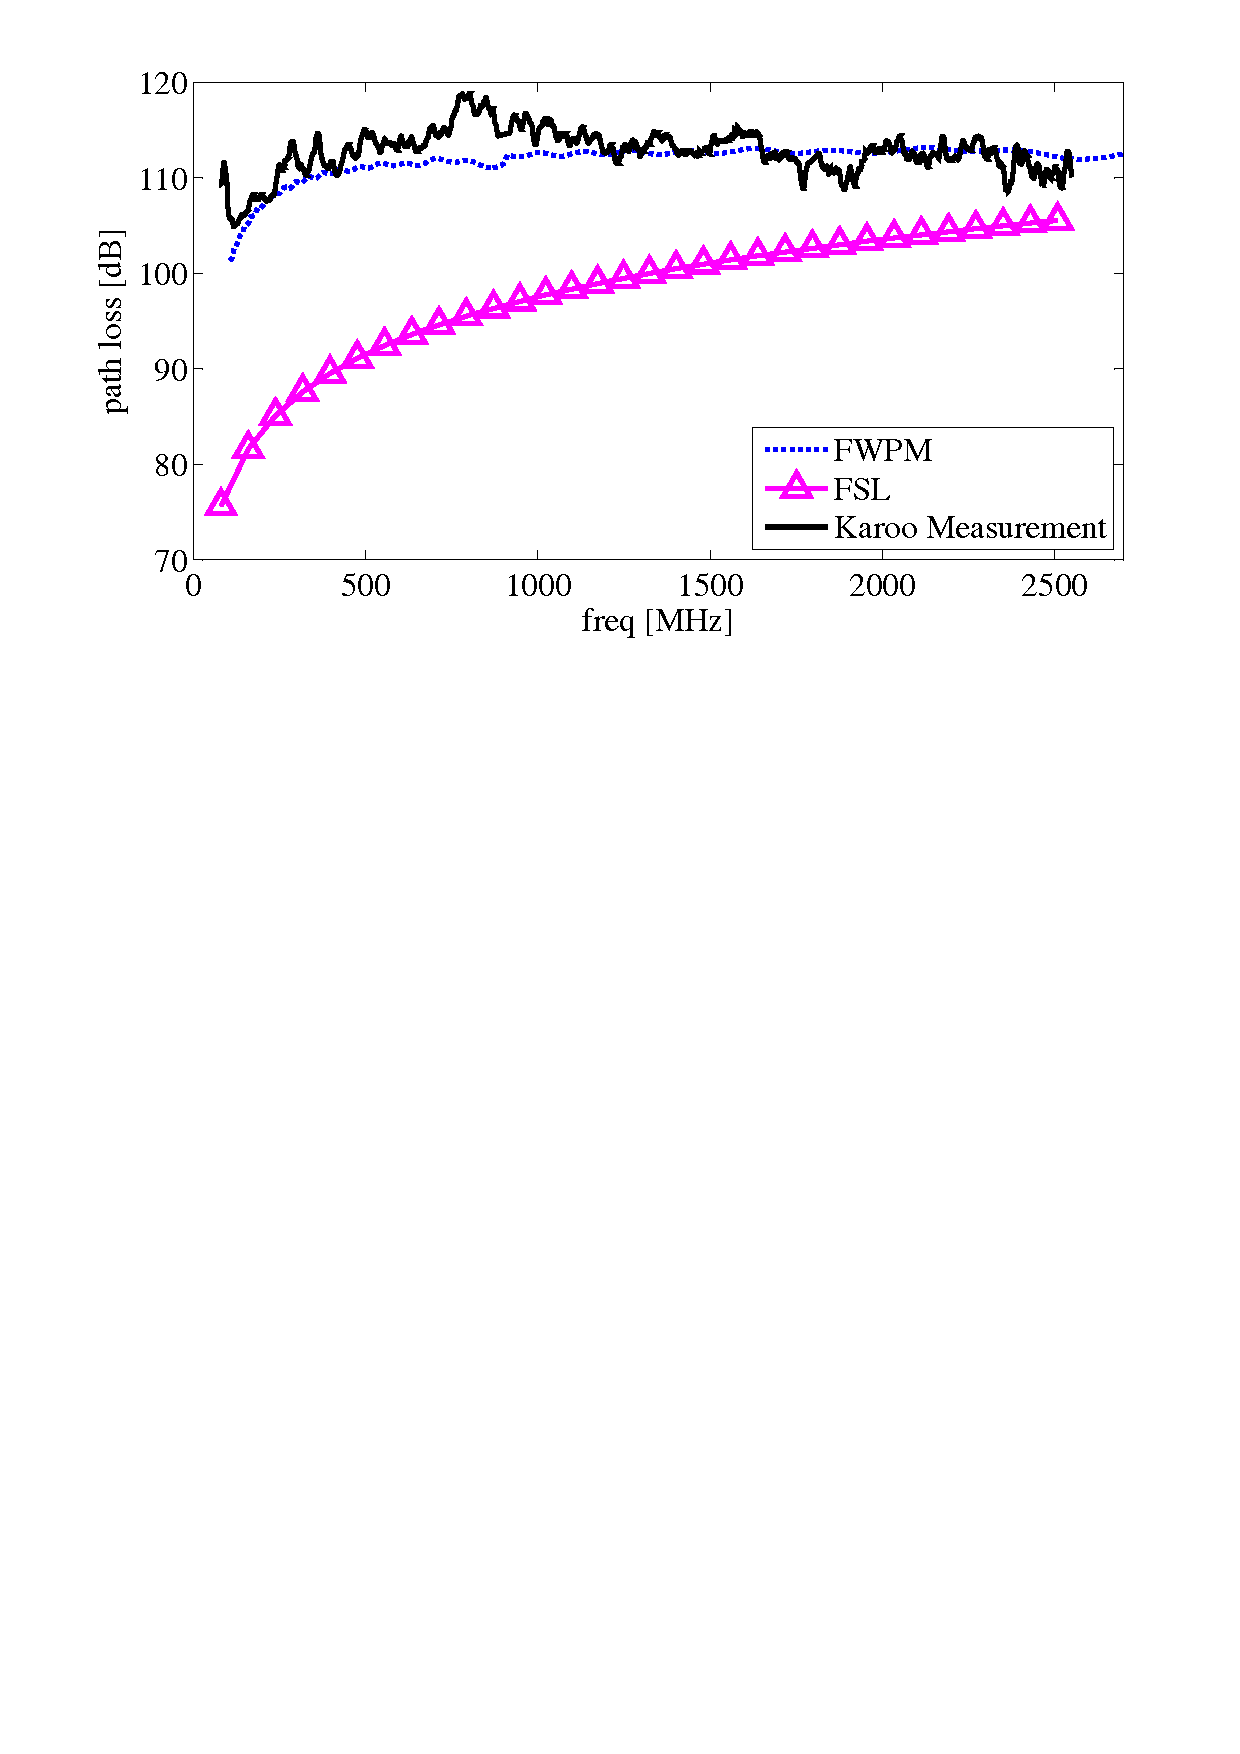
\includegraphics[width=0.32\linewidth]{Karoo_LH_1800m}%
	\label{fig:karoo_LH_1800m}}%
    \hfil
	\subfloat[]{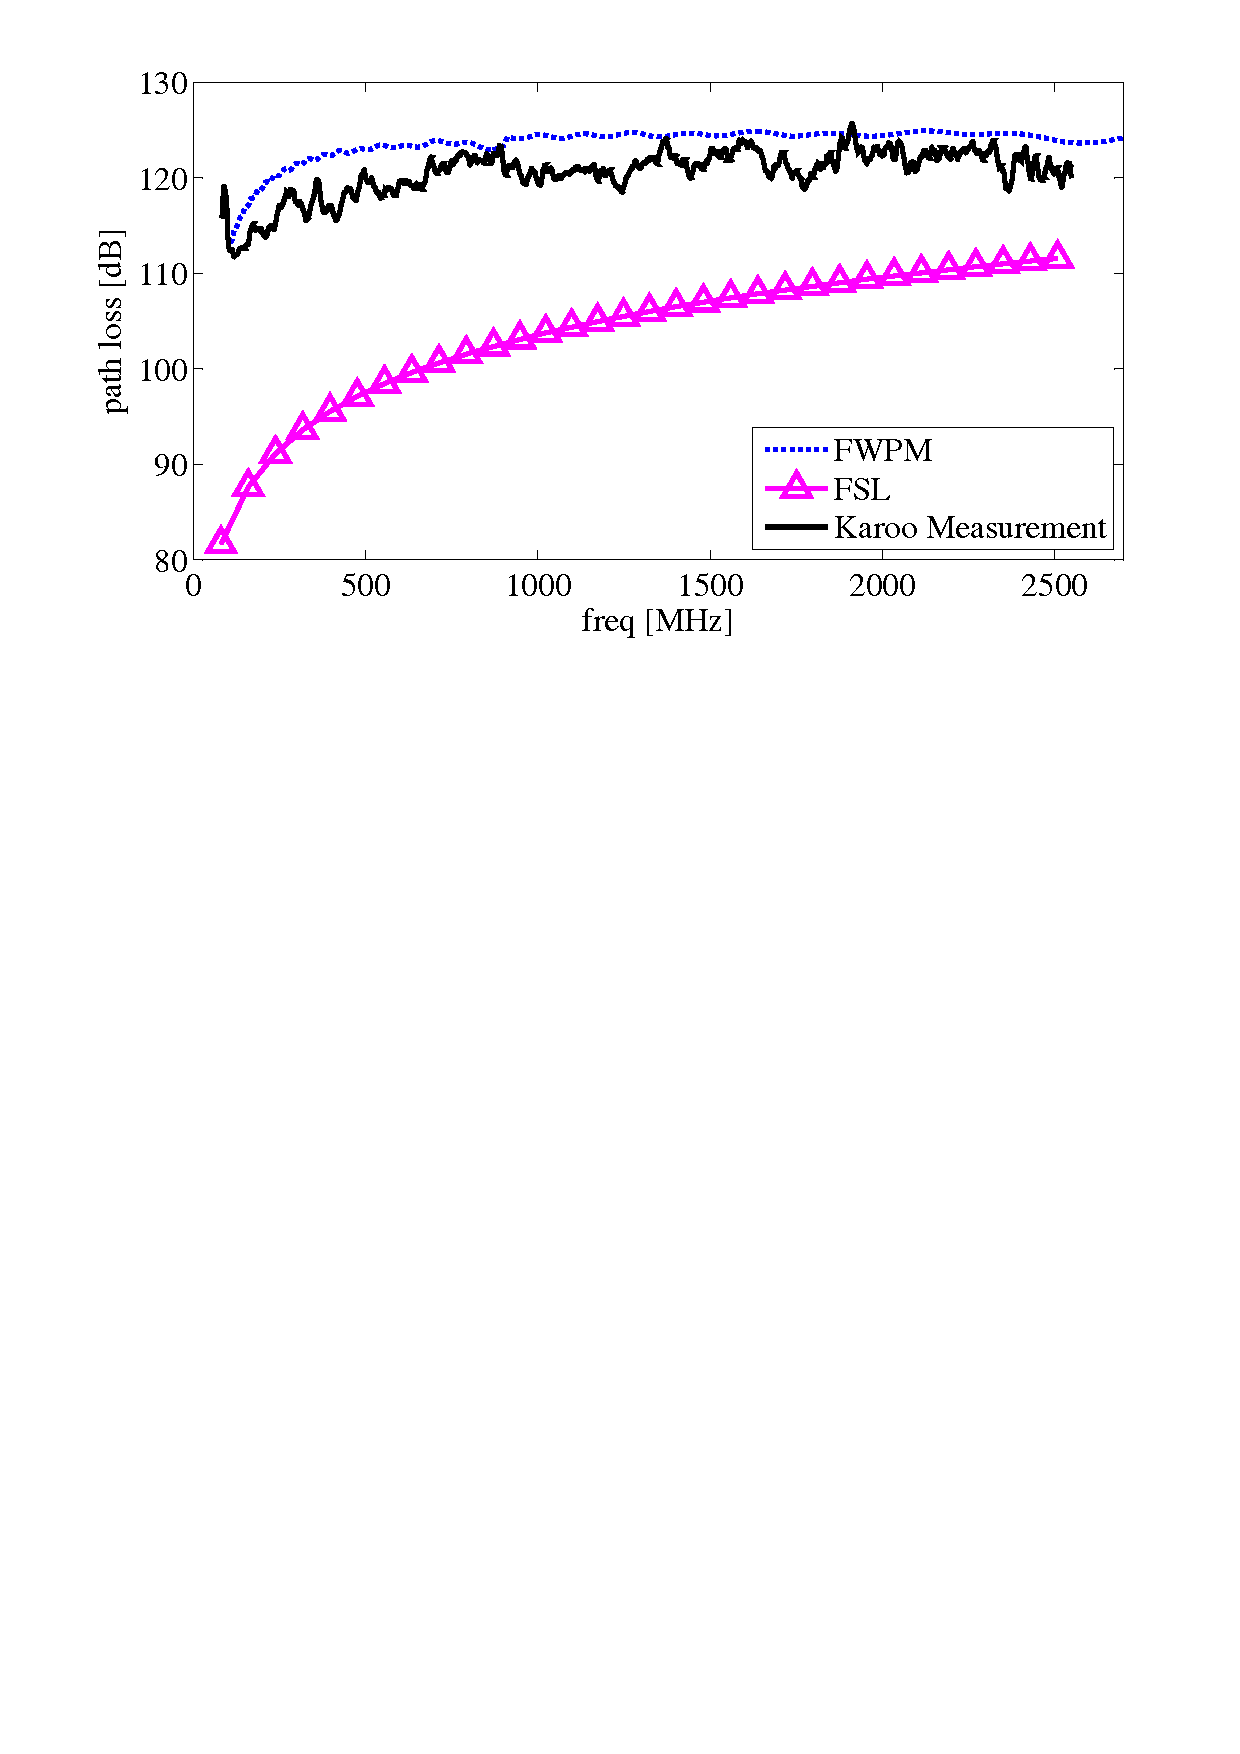
\includegraphics[width=0.32\linewidth]{Karoo_LH_3600m}%
	\label{fig:karoo_LH_3600m}}%
	\caption{Measured and predicted path loss in the Karoo: $h_t = \SI{7.5}{m}$, $h_r = \SI{2}{m}$ at T-R separations of \protect\subref{fig:karoo_LH_700m} \SI{700}{m}, \protect\subref{fig:karoo_LH_1800m} \SI{1800}{m} and \protect\subref{fig:karoo_LH_3600m} \SI{3600}{m}}%
	\label{fig:karoo_LH}%
\end{figure*}%
%\subsection{Statistical Error Analysis}
\begin{table*}[!ht]
	\centering
	\caption{Statistical Analysis on FWPM and FSL for Path Loss Predictions in the Karoo}
	\label{tb:stats2}
	\renewcommand{\arraystretch}{1.3}
	\setlength{\tabcolsep}{3pt}
	\begin{tabular*}{\linewidth}{ @{\extracolsep{\fill}} l*{10}c @{}}\toprule
		\multicolumn{11}{c}{Case I: $h_t = \SI{5}{m}$, $h_r = \SI{2}{m}$} \\    \midrule
		$d_m$& \multicolumn{2}{c}{Prediction Error, $\bar\varepsilon$} & \multicolumn{2}{c}{RMSE [\SI{}{dB}]} & \multicolumn{2}{c}{Relative Error} & \multicolumn{2}{c}{Accuracy} & \multicolumn{2}{c}{Corr Coefficient, $\rho$} \\ \cmidrule{1-1} \cmidrule{2-3} \cmidrule{4-5} \cmidrule{6-7} \cmidrule{8-9} \cmidrule{10-11}
		[\SI{}{m}]     & FWPM  & FSL   & FWPM  & FSL   & FWPM  & FSL   & FWPM  & FSL   & FWPM  & FSL \\
		\cmidrule{1-1} \cmidrule{2-3} \cmidrule{4-5} \cmidrule{6-7} \cmidrule{8-9} \cmidrule{10-11}
        50    & 1.31  & 6.13  & 3.33  & 6.97  & 0.034 & 0.080 & 96.60 & 92.01 & 0.956 & 0.979 \\
        200   & -0.05 & 3.18  & 2.11  & 3.88  & 0.018 & 0.043 & 98.19 & 95.75 & 0.951 & 0.944 \\
        700   & -1.30 & 7.73  & 2.25  & 9.25  & 0.016 & 0.081 & 98.38 & 91.86 & 0.783 & 0.702 \\
        1800  & -1.01 & 15.68 & 2.68  & 17.12 & 0.020 & 0.138 & 98.04 & 86.22 & 0.338 & 0.029 \\
        3600  & -4.67 & 17.91 & 5.05  & 18.88 & 0.039 & 0.147 & 96.06 & 85.28 & 0.616 & 0.512 \\ \cmidrule{1-1} \cmidrule{2-3} \cmidrule{4-5} \cmidrule{6-7} \cmidrule{8-9} \cmidrule{10-11}
        mean 1 & -0.02 & 5.68  & 2.56  & 6.70  & 0.023 & 0.068 & 97.72 & 93.21 & 0.896 & 0.875 \\
        mean 2 & -1.15 & 10.13 & 3.08  & 11.22 & 0.025 & 0.098 & 97.45 & 90.23 & 0.729 & 0.633 \\ \midrule
		\multicolumn{11}{c}{Case II: $h_t = \SI{7.5}{m}$, $h_r = \SI{2}{m}$} \\ \midrule
		50    & 1.89  & 7.40  & 5.06  & 8.94  & 0.056 & 0.094 & 94.43 & 90.55 & 0.966 & 0.977 \\
        200   & -0.20 & 5.35  & 4.40  & 7.89  & 0.036 & 0.059 & 96.43 & 94.10 & 0.929 & 0.892 \\
        700   & -0.41 & 6.21  & 2.53  & 7.34  & 0.017 & 0.067 & 98.28 & 93.28 & 0.802 & 0.857 \\
        1800  & 0.96  & 14.82 & 2.38  & 16.20 & 0.016 & 0.131 & 98.39 & 86.87 & 0.487 & 0.238 \\
        3600  & -3.12 & 16.56 & 3.47  & 17.26 & 0.026 & 0.138 & 97.38 & 86.21 & 0.792 & 0.819 \\ \cmidrule{1-1} \cmidrule{2-3} \cmidrule{4-5} \cmidrule{6-7} \cmidrule{8-9} \cmidrule{10-11}
        mean 1 & 0.43  & 6.32  & 3.99  & 8.06  & 0.036 & 0.074 & 96.38 & 92.64 & 0.899 & 0.909 \\
        mean 2 & -0.18 & 10.07 & 3.57  & 11.53 & 0.030 & 0.098 & 96.98 & 90.20 & 0.795 & 0.757 \\
		\bottomrule
	\end{tabular*}%
\end{table*}%
%

Fig \ref{fig:reflect_grazing} shows the magnitude of the Fresnel reflection coefficient as a function of incidence angle $\psi$ (dotted line) as well as the dependence of $\psi$ on distance (solid line) for $h_t=\SI{5}{m}$. Beyond about \SI{1}{km} the angle of incidence is negligibly small so that the Fresnel reflection coefficients are independent of complex permittivity and a PEC is approximated. That is, grazing angles yield a reflection coefficient of \num{-1} as predicted by equation (\ref{eq:Rv}), indicating a phase shift of $180^\circ$ which is typically associated with overlap and cancellation of the direct and reflected waves. It is plausible that the relative `flattening' of the path loss curves at \SI{700}{}, \SI{1800}{} and \SI{3600}{m} is due to this effect which is most pronounced at the higher frequencies. %A quasi-Brewster angle is encountered at $5.7^\circ$
%
\begin{figure} %[!ht]
	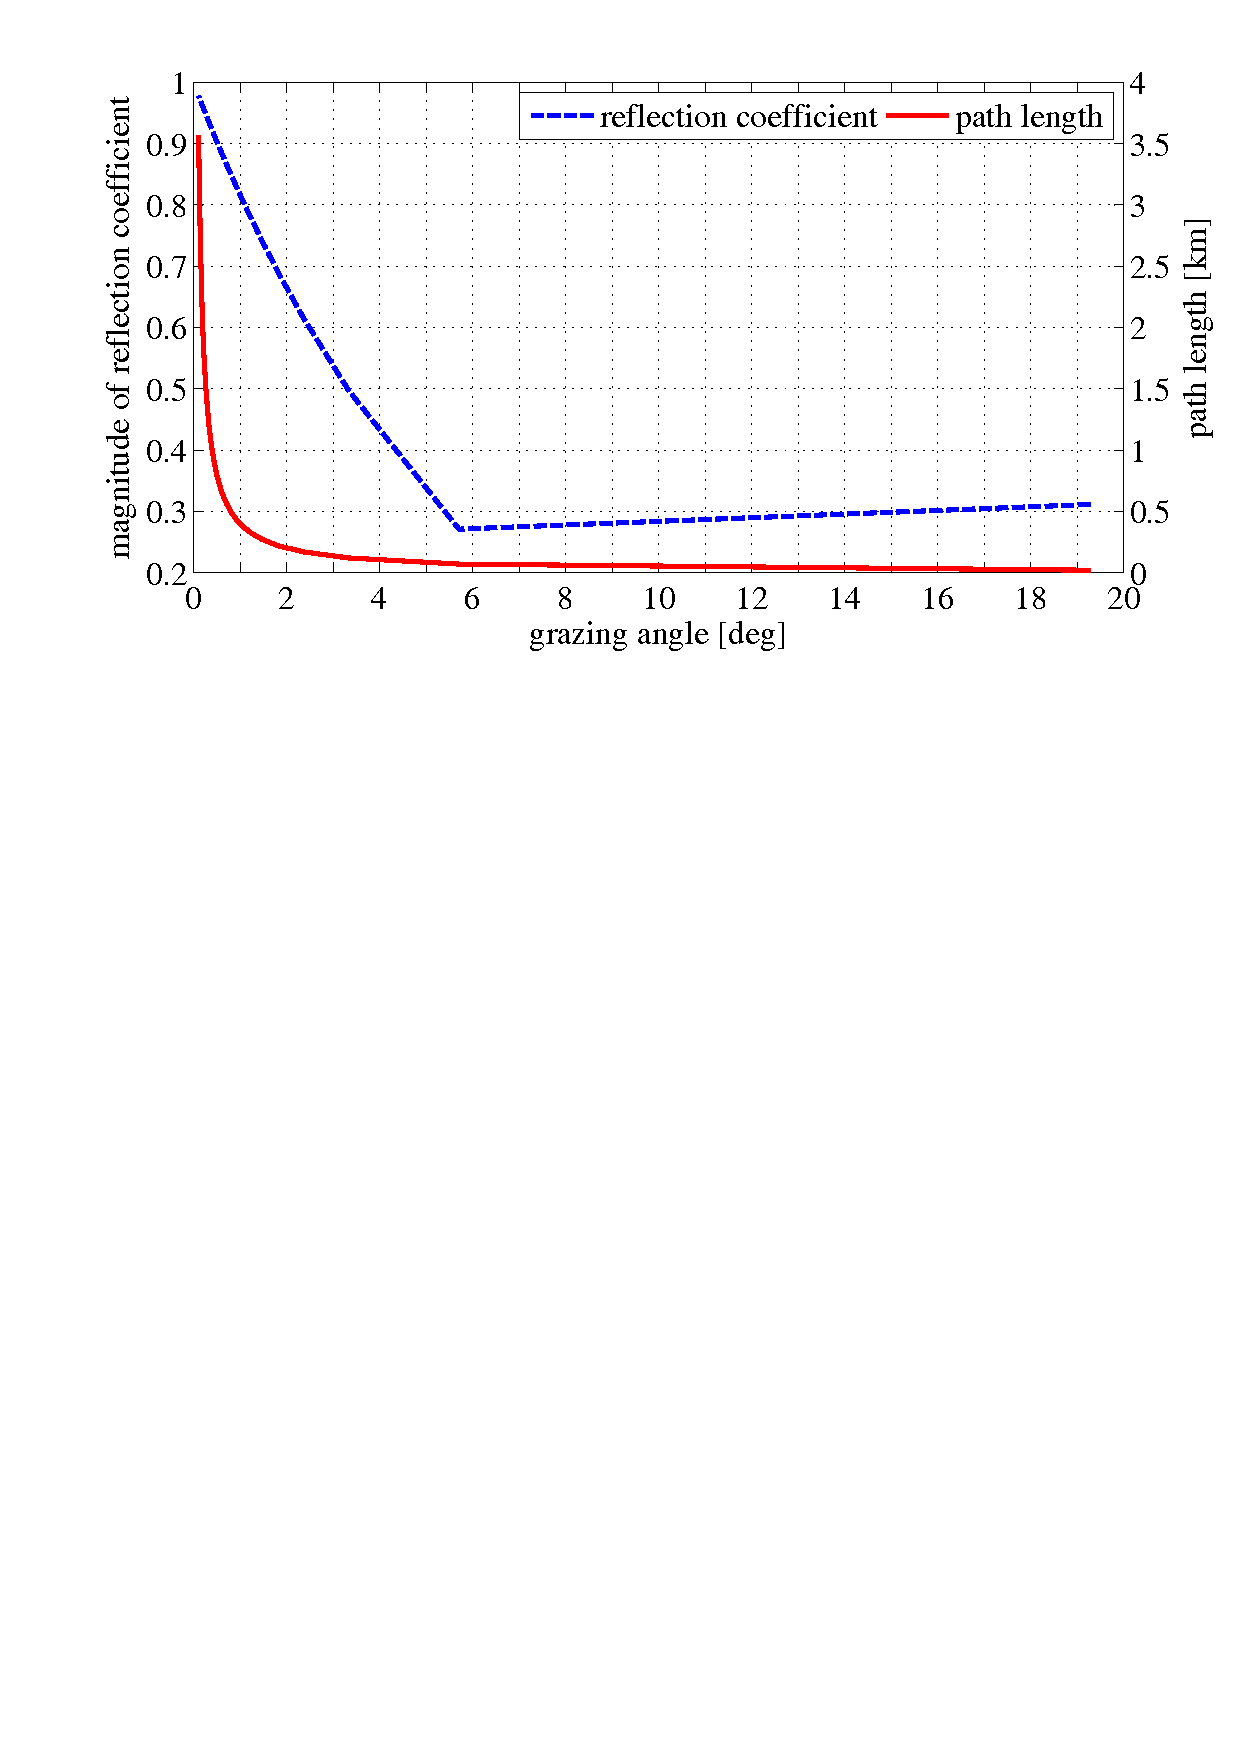
\includegraphics[width=\linewidth]{ground_reflection_coefficient_grazing_angle}
	\caption{Fresnel reflection coefficient and the variation of grazing angle with distance}
	\label{fig:reflect_grazing}
\end{figure} %
%
\section{Conclusion}\label{Conclusion}
In the Full Wave Propagation Model (FWPM) we have illustrated the implementation of an existing MoM-based code (FEKO) to predict path loss. The novelty in our work lies in the recreation of a real world measurement scenario wherein antenna characteristics and the influence of the earth are inherently accounted for. Although applied assuming a flat ground, statistical analysis on the FWPM predictions of path loss in the Karoo yielded an impressively low RMSE of $<\SI{4}{dB}$. The ability of the FWPM to model propagation over obstacles illustrates the versatility of the method to incorporate more sophisticated scenarios. This has the potential to facilitate easier development of `loss' maps and would be a vital tool for investigating coupling mechanisms, particularly in respect of facilities like MeerKAT. % On the other hand, although free space loss predictions fall within acceptable error margins below \SI{1}{km}, the prediction accuracy is unsatisfactory.\\
%This study suggests that the Karoo soil is good rather than bad ground as per the general categorization of types of surfaces.

\section*{Acknowledgement}
The financial assistance of the South African SKA Project (SKA SA) towards this research is hereby acknowledged. Opinions expressed and conclusions arrived at are those of the author and are not necessarily to be attributed to the SKA SA. (\url{www.ska.ac.za})\\
The authors thank EMC consultants MESA Solutions for sharing data and engaging in meaningful discussion. Special thanks to Anneke Bester for technical support during measurements in Stellenbosch. 

\bibliographystyle{IEEEtran}
\bibliography{IEEEabrv,tj_Journ_paper_refs}

\begin{IEEEbiography}[{
\includegraphics[width=1in,height=1.25in,clip,keepaspectratio]{./tj2.jpg}}]{Temwani J. Phiri}
Biography text here.
\end{IEEEbiography}

%% if you will not have a photo at all:
%\begin{IEEEbiographynophoto}{John Doe}
%Biography text here.
%\end{IEEEbiographynophoto}

% insert where needed to balance the two columns on the last page with
% biographies
%\newpage

\begin{IEEEbiography}[{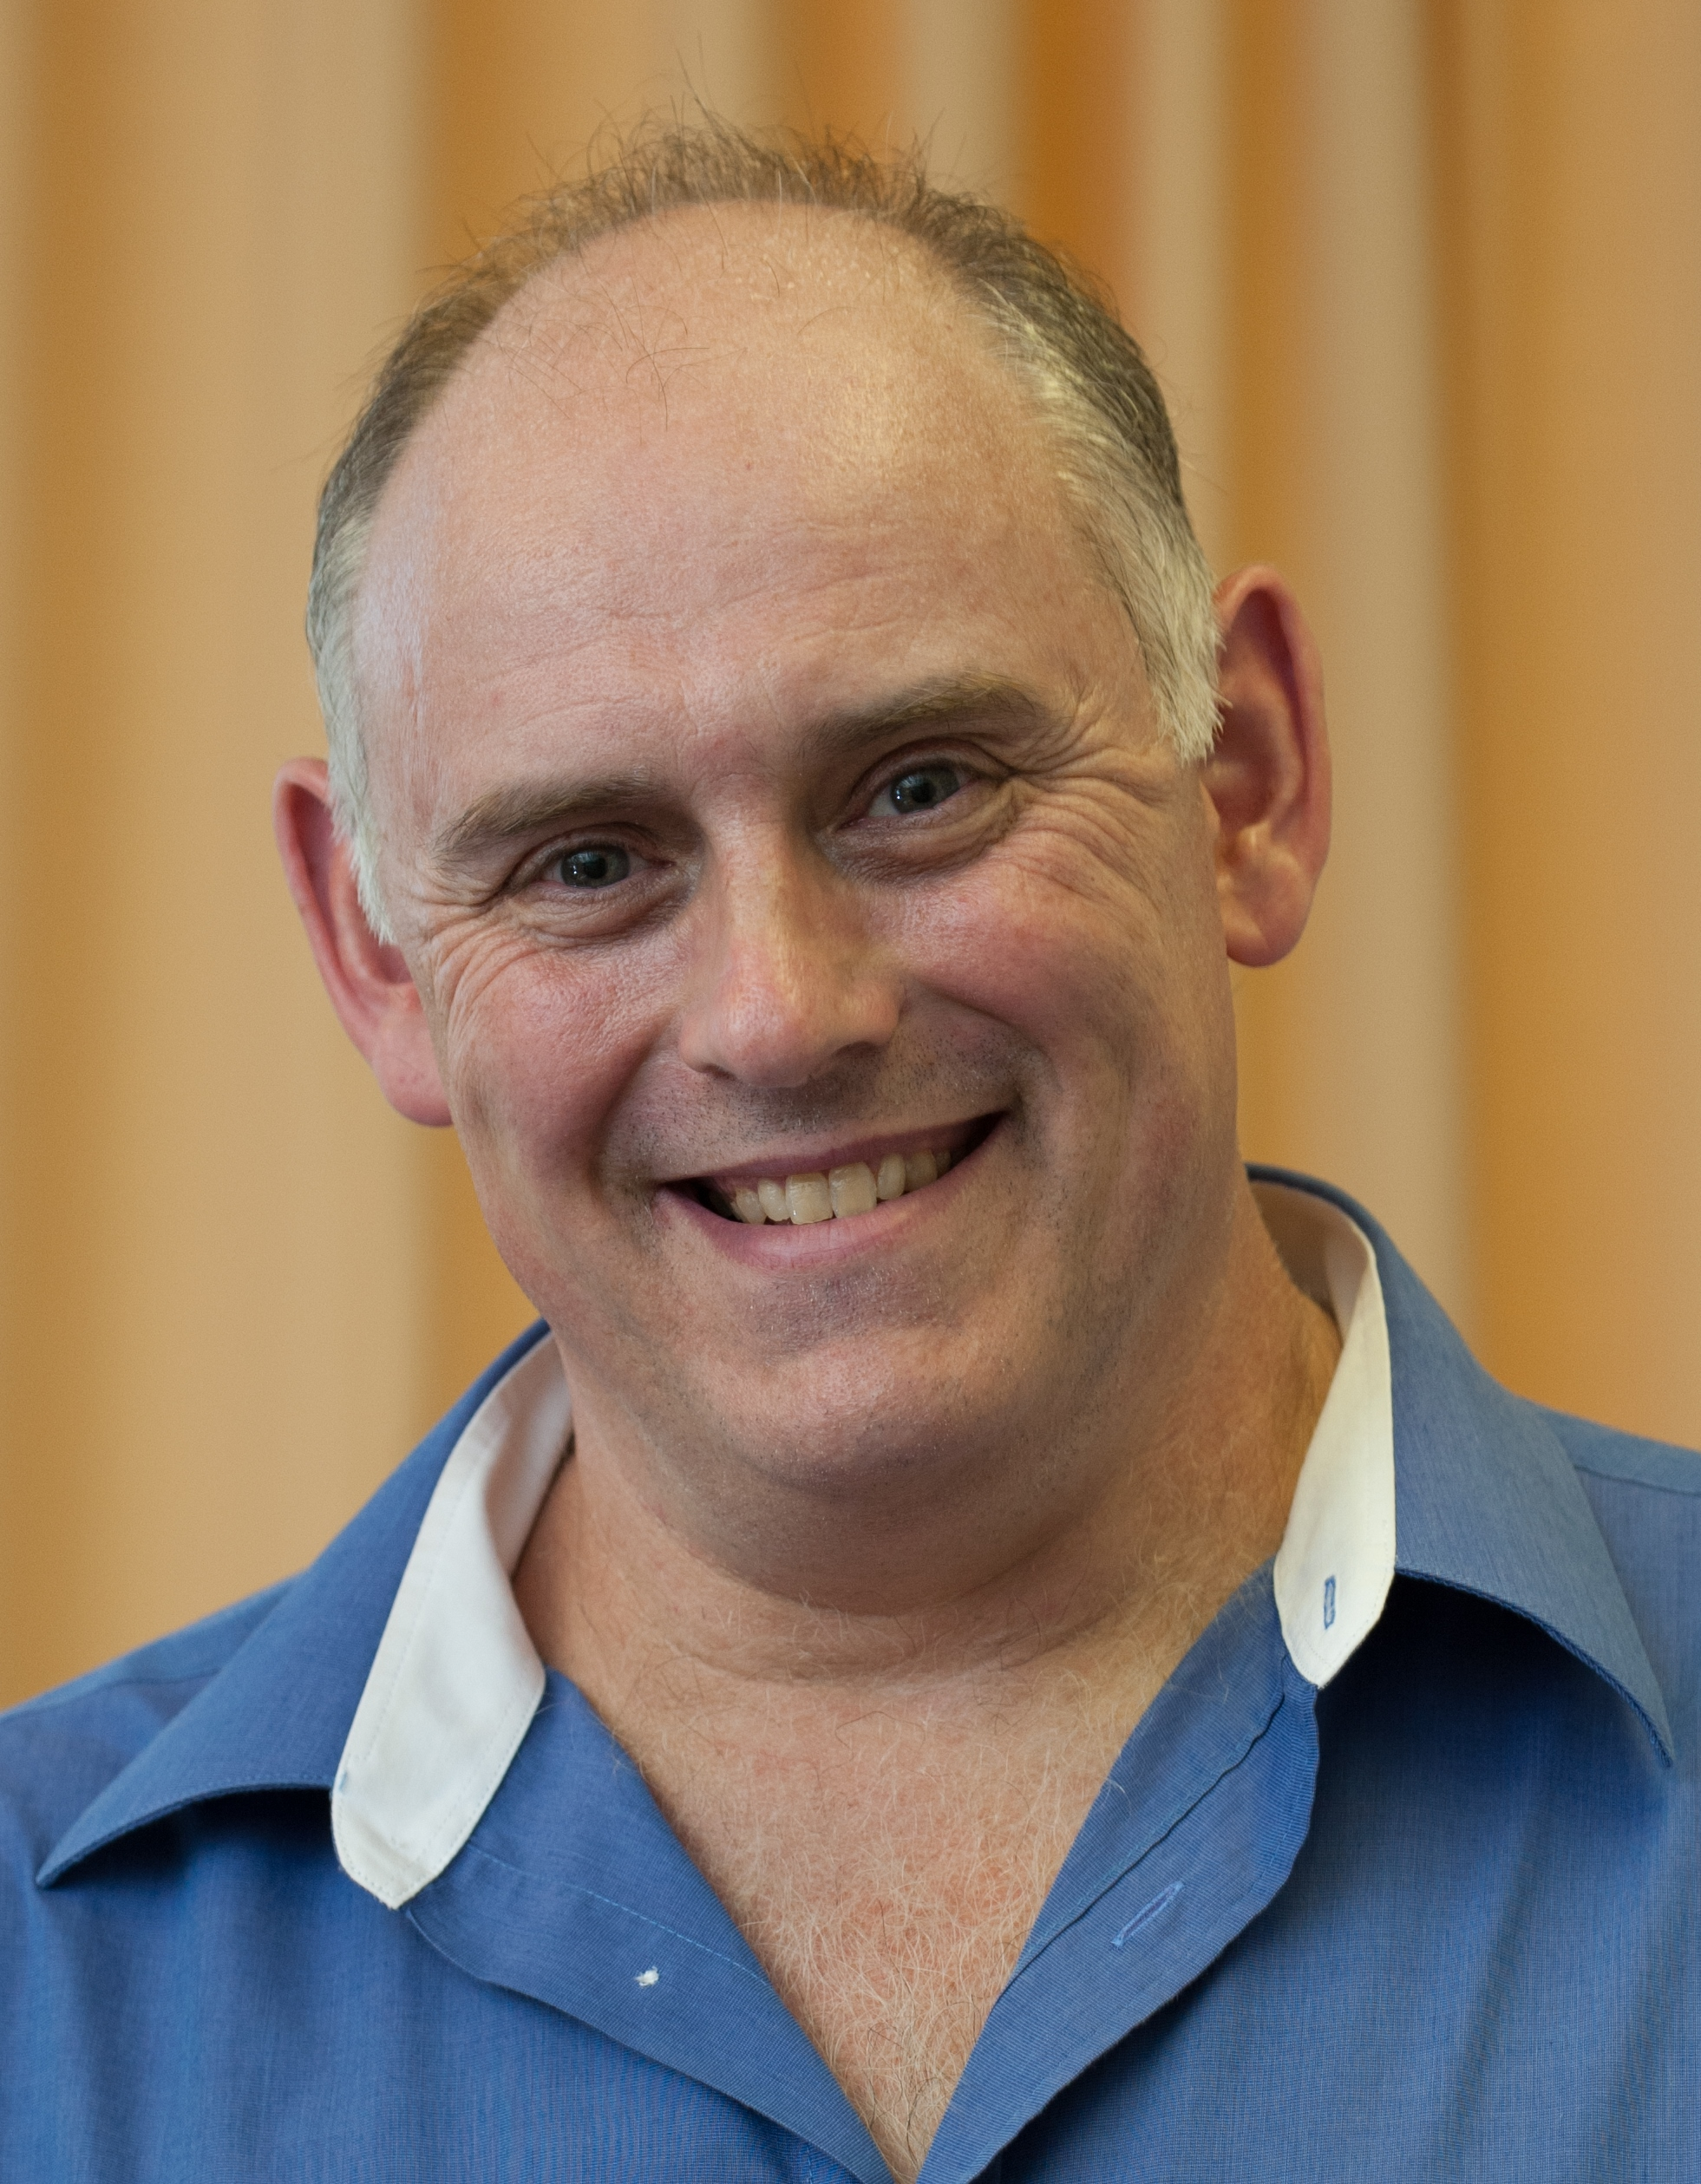
\includegraphics[width=1in,height=1.25in,clip,keepaspectratio]{./Davidson.jpg}}]{David B. Davidson}
Biography text here.
\end{IEEEbiography}

% You can push biographies down or up by placing
% a \vfill before or after them. The appropriate
% use of \vfill depends on what kind of text is
% on the last page and whether or not the columns
% are being equalized.

%\vfill

\begin{IEEEbiography}[{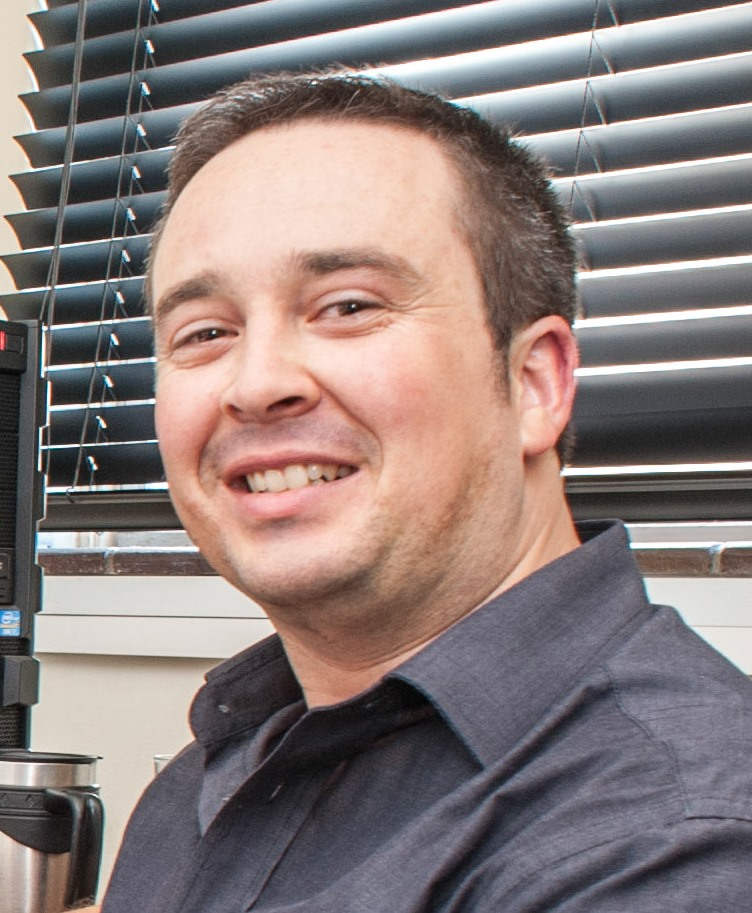
\includegraphics[width=1in,height=1.25in,clip,keepaspectratio]{./Wiid.jpg}}]{P. Gideon Wiid}
Biography text here.
\end{IEEEbiography}

% Can be used to pull up biographies so that the bottom of the last one
% is flush with the other column.
%\enlargethispage{-5in}
\end{document}